
In this section, which can for the most part be read independently of the rest of the paper, we investigate the fate of the Kervaire invariant one classes in the Adams spectral sequence.
The celebrated Hill--Hopkins--Ravenel theorem on Kervaire invariant one tells us that $h_j^2$ supports a non-trivial Adams differential for every $j \geq 7$ \cite{HHR}. However, their work provides no further identifying information about these differentials.\footnote{For example, it remains possible that the lengths of these differentials grows without bound as $j$ increases.}
% Although the authors find it unlikely that this is the case, we must acknowledge that if this is the case, then it is probable that we will never know their precise length or target classes.}
As a corollary of our study of these classes we provide a new lower bound on the length of the HHR differentials, showing that $ d_4(h_j^2) = 0 $.

It is in this section that the distinction between $\Theta_j$, $\theta_j$ and $h_j^2$ becomes important and for this reason we pause to introduce to the reader of our conventions.
  %For the attentive reader who has already noticed our varying use of $\Theta_j$ and $\theta_j$ we provide the following explanation.
  We use $\Theta_j$ for the Kervaire invariant one classes in the classical stable homotopy groups of spheres.
  We use $h_j^2$ for the class on the Adams $E_2$-page.
  We use $\theta_j$ for a choice of class in the synthetic homotopy groups of $\clambda^k$ (which exists when $h_j^2$ survives to the $E_{k+1}$-page of the Adams spectral sequence).

We obtain our lower bound by revisiting one of the most promising proposals for constructing $\Theta_j$, the inductive approach of Barratt--Jones--Mahowald \cite{Inductive}. %\todo{is this the right attribution?}.
The crux of this approach is a construction which proceeds
\[ \begin{pmatrix} \Theta_j \text{ exists } \\ 2\Theta_j  = 0 \\ \Theta_j^2 = 0 \end{pmatrix} \Longrightarrow \begin{pmatrix} \Theta_{j+1} \text{ exists } \\ 2\Theta_{j+1} = 0 \end{pmatrix}. \]

In light of the HHR theorem this approach must break down at some point, meaning at least one of $\Theta_5^2$ or $\Theta_6^2$ is non-zero. The idea we pursue in this section is that it should be possible to run the inductive approach internal to the Adams spectral sequence on a fixed page. The main result of this section, \Cref{thm:inductive}, can be informally summarized as saying that,
\[ \begin{pmatrix} \theta_j \text{ survives to the } E_r \text{-page }\\ 2\theta_j = 0 \text{ on the } E_r \text{-page } \\ \theta_j^2 = 0 \text{ on the } E_{r-2} \text{-page } \end{pmatrix} \Longrightarrow \begin{pmatrix} \theta_j \text{ survives to the } E_r \text{-page }\\ 2\theta_j = 0 \text{ on the } E_r \text{-page } \end{pmatrix}. \]

The power of this result lies in the fact that the inductive hypothesis we must verify lies 2 pages prior to the conclusion. This means that if we proceed by induction on $r$ (rather than induction on $j$) the classes $\theta_j^2$ are already defined for all $j$ at the outset. This opens the possibility that $\theta_j^2$ might be identified on the Adams $E_r$-page simultaneously for all $j$ and that being non-zero we might, then read off the HHR differentials. In order to make the expected outcome as concrete and precise as possible we make the following conjecture, which is a special case of Conjecture~\ref{conj: stable length}.

\begin{cnj}[Uniform Kervaire differentials conjecture]
  There exists a $Sq^0$-family of classes $(\mathrm{HHR})_j$ on the Adams $E_2$-page (defined for $j \gg 0$) and another class $x$ on the $E_2$-page such that
  \[ d_r(h_j^2) = x \cdot (\mathrm{HHR})_j \neq 0. \]
\end{cnj}

In order to make the idea of ``working on a fixed page of the Adams spectral sequence'' rigorous we will work in the category of $\F_2$-synthetic spectra introduced in \cite{Pstragowski}. In the first subsection of this section we provide a lightning introduction to this category and its connection to the Adams spectral sequence. In the second subsection we run the Barratt--Jones--Mahowald inductive argument internal to the category of $\F_2$-synthetic spectra. In the final subsection we investigate a certain product related to the differential on $h_j^3$.

%\begin{rmk}
%  It is in this section that the distinction between $\Theta_j$, $\theta_j$ and $h_j^2$ becomes important and for this reason we pause to remind the reader of our conventions.
  %For the attentive reader who has already noticed our varying use of $\Theta_j$ and $\theta_j$ we provide the following explanation.
%  We use $\Theta_j$ for the Kervaire invariant one classes in the stable homotopy groups of spheres.
%  We use $h_j^2$ for the class on the Adams $E_2$-page.
%  We use $\theta_j$ for a choice of class in the synthetic homotopy groups of $\clambda^k$ (which exists when $h_j^2$ survives to the $E_{k+1}$-page of the Adams spectral sequence).
%\end{rmk}


% ---------------------------------------------------------------------------------%
% ---------------------------------------------------------------------------------%
\subsection{A lightning introduction to synthetic spectra}\ 
\label{subsec:syn-intro}

% In order to prove the main results of this section we will need to be able to understand how the Adams filtration and Adams differentials interact with power operations. 

% \todo{This needs to be rewritten}


% This subject begins with work of Adams, Barratt and Mahowald and attained a relatively stable form with Bruner's foundational work in \cite{BMMS}. Pairing this with a modern understanding of the Adams spectral sequence as provided by Pstragowski's category of synthetic spectra \cite{Pstragowski} we will obtain a robust tool for manipulating differentials in Adams type spectral sequences.

In this subsection we provide a minimal introduction to the category of $\F_2$-synthetic spectra.
For a more complete introduction focusing on the construction of this category see \cite{Pstragowski}.
For a short introduction tailored to using synthetic spectra for computational purposes see \cite[Sections 9 and A]{boundaries}.
For a more comprehensive account of synthetic homotopy theory see the (forthcoming) book \cite{cookware}. Since our main application is only in the case of $\F_2$ we will stick to this case throughout our exposition.

% ---------------------------------------------------------------------------------%
\subsubsection{Synthetic spectra}\hfill

Let $\mathrm{Stable}_{\A}$ be Hovey's stable $\infty$-category of comodules \cite{Hovey} over the Steenrod algebra $\A$.

\begin{cnstr}[Pstr\k{a}gowski]\label{cnstr:syn}
  There is a stable, presentably symmetric monoidal $\infty$-category $\mathrm{Syn}_{\F_2}$
  which fits into a diagram of symmetric monoidal functors
  \begin{center}
    \begin{tikzcd}
      & \Sp \ar[ddl, swap, "1", bend right] \ar[d, "\nu"] \ar[ddr, "(\F_2)_*(-)", bend left] & \\
      & \mathrm{Syn}_{\F_2} \ar[dl, "\lambda^{-1}"] \ar[dr, "- \otimes \clambda"'] & \\
      \Sp & & \mathrm{Stable}_{\A}
    \end{tikzcd}
  \end{center}
  with the following properties:
  \begin{enumerate}
  \item $\nu$ commutes with filtered colimits and sends a cofiber sequence to a cofiber sequence if and only if it induces a short exact sequence on $\F_2$-homology.\footnote{This condition on cofiber sequences is exactly the minimal one so that we have a long exact sequence at the level of the Adams $E_2$-page.}
  \item The functors $- \otimes \clambda$ and $\lambda^{-1}$ each commute with colimits.%\footnote{We will return to the actual meaning of the recurring term $\lambda$ shortly.}.
  \item The functor $\lambda^{-1}$ is a localization. 
  \end{enumerate}  
\end{cnstr}
  
For each spectrum $X$ the object $\nu X$ records all information present in the Adams spectral sequence for $X$. In fact, one can reasonably think about the object $\nu X$ as \emph{being} the Adams spectral sequence for $X$.

% ---------------------------------------------------------------------------------%
\subsubsection{Synthetic homotopy groups}\hfill
 
Before we can justify our claim that $\nu X$ records the data present in the Adams spectral sequence for $X$ we will need to introduce a way to measure a synthetic spectrum.
For this our preferred method is via the \emph{bigraded synthetic homotopy groups} and the action of the canonical bigraded homotopy element $\lambda$ on them. For the reader familiar with motivic spectra over $\mathbb{C}$ this pattern should be relatively familiar.

\begin{dfn}[{\cite[Definitions 4.6 and 4.9]{Pstragowski}}]
  The \emph{bigraded synthetic sphere} $\Ss^{k,s}$ is defined\footnote{We warn the reader that our conventions differ from those in some previous references. With the conventions used here the two indices of $\Ss^{k,s}$ are the $x$ and $y$ coordinates in an Adams chart. We have found that in practice these are the most user-friendly conventions.} to be $\Sigma^{-s} \nu S^{k+s}$.
  As is standard we will omit the superscripts in the case $(0,0)$, using the symbol $\Ss$ for the monoidal unit of $\Syn_{\F_2}$.
  For any synthetic spectrum $X$, the \emph{bigraded homotopy group} $\pi_{k,s}(X)$ is defined to be the abelian group of homotopy classes of maps with source $\Ss^{k,s}$ and target $X$.
\end{dfn}
  
\begin{dfn}[{\cite[Definition 4.27]{Pstragowski}}]
  For each spectrum $X$ we have an assembly map $\Sigma \nu X \to \nu \Sigma X$.
  In the case of $S^{-1}$ this provides us with a canonical map\footnote{Typically this class is referred to as $\tau$. Since we make use of both the synthetic and motivic categories, we denote it by $\lambda$ instead.}%figure prominently in this paper we have decided to break with standard notation in order to disambiguate.}
  \[ \lambda : \Ss^{0,-1} \simeq \Sigma \nu S^{-1} \longrightarrow \nu \Sigma S^{-1} \simeq \Ss^{0,0}. \]
  % which we will call $\lambda$.
\end{dfn}

The class $\lambda \in \pi_{0,-1} \Ss$ and its behavior is the most important feature of the category of synthetic spectra. As an example say that $X$ is \emph{$\lambda$-invertible} (\cite[Definition 4.32]{Pstragowski}) if the map $$\lambda: \Sigma^{0,-1} X \to X$$ is an equivalence. Then, the symmetric monoidal localization functor associated to the map $\lambda$ is the functor $\lambda^{-1}$ given above. In particular, the full subcategory of $\lambda$-invertible objects is equivalent to the category of spectra.
At the opposite extreme,
let the symbol $\clambda$ denotes the cofiber of $\lambda$,
then we have a simple description of the homotopy groups of $\clambda \otimes X$. 

\begin{lem}[{\cite[Lemma 4.56]{Pstragowski}}] \label{lem:ctau-E2}
  For any spectrum $X$, there is a natural isomorphism of bigraded abelian groups
  \[ \pi_{t-s,s}(\clambda \otimes \nu X) \cong \Ext_{\A}^{s,t}(\F_2,(\F_2)_*X) \]
  between homotopy groups mod $\lambda$ and the $E_2$-page of the Adams spectral sequence for $X$.
\end{lem}

% For the moment we also remark that $\clambda$ can be given a commutative algebra structure and that we will return to this point later.

In fact, this lemma is only a prelude to \cite[Theorem 9.19]{boundaries} which gives a precise translation\footnote{Again we warn the reader that our grading differs by a shearing from those used in loc. cit. That said, $k$ and $s$ are the same.} between Adams spectral sequence data for $X$ and bigraded synthetic homotopy groups for $\nu X$. Again for the readers familiar with motivic spectra over $\mathbb{C}$ this pattern should be relatively familiar.

% \begin{thm}[{\cite[Theorem 9.19]{boundaries}}] \label{thm:synthetic-Adams}
%   Let $X$ denote an $F_2$-nilpotent complete spectrum with strongly convergent Adams spectral sequence.
%   The bigraded homotopy groups of $\nu X$ admit the following description.

%   Suppose $x$ is a class in topological degree $k$ and filtration $s$ of the $E_2$-page of the Adams spectral sequence for $X$. The following are equivalent:
%   \begin{itemize}
%   \item[(1a)] Each of the differentials $d_2$,...,$d_r$ vanish on $x$.
%   \item[(1b)] $x$, viewed as an element of $\pi_{k,s}(\clambda \otimes \nu X)$, lifts to $\pi_{k,s}(\clambda^r \otimes \nu X)$.
%   \item[(1c)] $x$ admits a lift to $\pi_{k,s}(\clambda^r \otimes \nu X)$ whose image under the $\lambda$-Bockstein
%   \[ \clambda^r \otimes \nu X \to \Sigma^{1,-r-1} \clambda \otimes \nu X \]
%   is equal to $-d_{r+1}(x)$.
%   \end{itemize}

%   If we moreover assume that $x$ is a permanent cycle, then there exists a (not necessarily unique) lift of $x$ along the map
%   $\pi_{k,s}(\nu X) \to \pi_{k,s}(\clambda \otimes \nu X)$.  For any such lift, $\wt{x}$, the following statements are true:
%   \begin{itemize}
%   \item[(2a)] If $x$ survives to the $E_{r+1}$-page, then $\lambda^{r-1} \wt{x} \neq 0$.
%   \item[(2b)] If $x$ survives to the $E_\infty$-page, then the image of $\wt{x}$ in $\pi_{k} (X)$ is of Adams filtration $s$ and detected by $x$ in the Adams spectral sequence.    
%   \end{itemize}
%   Furthermore, there always exists a choice of lift $\wt{x}$ satisfying additional properties:
%   \begin{itemize}
%   \item[(3a)] If $x$ is the target of a $d_{r+1}$-differential, then we may choose $\wt{x}$ so that $\lambda^r \wt{x} = 0$.
%   \item[(3b)] If $x$ survives to the $E_\infty$-page, and $\alpha \in \pi_k X$ is detected by $x$, then we may choose $\wt{x}$ so that
%     $\lambda^{-1} \wt{x} = \alpha$. In this case we will often write $\wt{\alpha}$ for $\wt{x}$.
%   \end{itemize}
%   Finally, essentially all elements of the bigraded homotopy groups arise via this theorem in the following sense:
%   \begin{itemize}
%   \item[(4)] Fix any collection of $\wt{x}$ (not necessarily chosen according to (3)) such that the $x$ span the permanent cycles in topological degree $k$.  Then the $\lambda$-adic completion of the $\Z[\lambda]$-submodule of $\pi_{k,*}(\nu X)$ generated by those $\wt{x}$ is equal to $\pi_{k,*} (\nu X)$.
%   \end{itemize}
% \end{thm}

% ---------------------------------------------------------------------------------%

%---------------------------------------------------------------------------------%
\subsubsection{The $\lambda$-bockstein tower}\hfill

With the class $\lambda$ in hand we can refine our understanding of the diagram in \Cref{cnstr:syn}.

\begin{thm}[Pstr\k{a}gowski] \label{thm:tau-inv}\ 

  \begin{enumerate}
  \item The cofiber of $\lambda$, which we denote $\clambda$, admits the structure of a commutative algebra in $\Syn_{\F_p}$.
  \item There is a natural symmetric monoidal equivalence
    \[ \mathrm{Mod}(\Syn_{\F_p}; \clambda) \to \mathrm{Stable}_{\A}, \]
    from the stable $\infty$-category of modules over $\clambda$ to Hovey's stable $\infty$-category of comodules over the Steenrod algebra $\A$.
    The composite of $\nu$ with $\clambda \otimes - $ and this equivalence is naturally equivalent to the $\F_p$-homology functor.
  \end{enumerate}
\end{thm}

% \begin{rmk}
%   Echoing \cite[Remark 9.14]{boundaries} we point out that \Cref{thm:tau-inv} suggests the following algebro-geometric picture of the category of synthetic spectra:
%   $\Syn_{\F_p}$ is a family of categories over a copy of $\mathbb{A}^1$ with coordinate $\lambda$.
%   This family of categories is $\mathbb{G}_m$-equivariant and its fiber at $0$ is a category of comodules while the generic fiber is the category of spectra.
%   In this way we see that $\Syn_{\F_p}$ is a degeneration of $\Sp$ to an algebra central fiber\footnote{The reader should imagine this like one imagines a toric degeneration such as $(yt)^2 = x^3 + ax + b$ (with $t$ being the parameter).}.
% \end{rmk}

In fact, we can go beyond just $\clambda$ and study $\clambda^n$ for varying $n$.
To do this in a coherent way we will need \cite[Example C.15]{rmot} and the surrounding material.
As a consequence of this $\Syn_{\F_p}$ has the structure of a locally filtered category in the sense of \cite{rotation}
where the canonical shift map is $\lambda$.
Through this we make the following construction. %synthetic spectra inherit the following from the universal example of a locally filtered category (filtered spectra):

\begin{cnstr}\label{cnstr:bock-maps}
  The locally filtered structure on $\Syn_{\F_p}$ comes from a symmetric monoidal left adjoint
  \[ i : \Sp^{\Fil} \to \Syn_{\F_p} \]
where $\Sp^{\Fil}$ is the category of filtered spectra and $i$ sends the shifted sphere spectrum $S(1)$ to $\Ss^{0,1}$ (see \cite[Definition B.3]{rmot} for the definition of filtered spectra and the natural automorphism $(1)$).
  This provides us with a tower of commutative algebras
  \[ \Ss \to \cdots \to \clambda^3 \to \clambda^2 \to \clambda. \]
  Using $r_{n,m}$ to denote these restriction maps, we have cofiber sequences
  \[ \Sigma^{0,m-n}\clambda^{n-m} \xrightarrow{\underline{\lambda^{m}}}  \clambda^n \xrightarrow{r_{n,m}} \clambda^m \xrightarrow{\delta_{n,m}} \Sigma^{1, m-n-1}\clambda^{n-m}. \]
  \[ \Sigma^{0,-m}\Ss \xrightarrow{{\lambda^{m}}}  \Ss \xrightarrow{r_{m}} \clambda^m \xrightarrow{\delta_{m}} \Sigma^{1, -m-1} \Ss. \]
  % Note that since the maps $\delta_{n,m}$ encode Adams differentials their linearity over $\clambda^n$ implies a Liebniz rule for Adams differentials.   
\end{cnstr}

The commutative algebra structure on $\clambda^n$ provides us with a symmetric monoidal category of modules over this object. In view of the connection between the $\lambda$-bockstein and Adams differentials we think of the category of $\clambda^n$-modules as providing a way to work at the level of the Adams $E_{n+1}$-page.

\begin{wrn}
  Outside the $n=1$ case, 
  the bigraded homotopy groups of $\clambda^n$ are not literally given by the Adams $E_{n+1}$-page.
  Instead, thinking through the mechanics of the $\lambda$-bockstein spectral sequence one finds that there is a surjective map
  \[ \pi_{k,s}(\clambda^n) \longrightarrow E_{n+1}^{s, k+s} \]
  with kernel generated by the image of $\underline{\lambda}$ together with the $\lambda^{n-1}$-torsion classes. Here $\underline{\lambda}$ is the boundary map in the cofiber sequence in \Cref{cnstr:bock-maps} for $m=1, n \geq 2$.
\end{wrn}

%---------------------------------------------------------------------------------%
\subsubsection{Examples of synthetic homotopy groups}\hfill

%Although \cite[Theorem 9.19]{boundaries} gives a complete interpretation of the data in the Adams spectral sequence in terms of synthetic homotopy groups its statement is quite long and it takes some effort to digest properly. 
In order to prepare for later subsections we work through several examples of synthetic homotopy groups. Each of our examples will correspond to understanding a small region of the Adams spectral sequence for the sphere near $h_j^2$. Before proceeding, we suggest the reader new to synthetic spectra look at \cite[Section A.2]{boundaries} which works through an example chosen for its instructiveness in full detail.


\begin{sseqdata}[ name = thetaASS, xscale=1.25, yscale=1.25, x range = {-5}{0}, y range = {0}{5}, x tick step = 2, y tick step = 2, class labels = {left}, classes = fill, grid = crossword, Adams grading, lax degree]

  \class["h_j^2"](-2,2)
  \class(-2,3) \structline
  \class(-2,4) \structline
  \class(-2,5) \structline
  \class(-2,6) \structline
  \class(-2,7) \structline

  \class(-1,3) \structline(-2,2)
  \class(0,4) \structline
  \class(1,5) \structline 
  % \class(1,5) \structline \structline(-2,4)
  % \class(1,3) \structline(-2,2)
  % \class(1,4) \structline(-2,3) \structline \structline(1,5)
  
  \class["h_{j+1}"](-1,1)
  \class(-1,2) \structline
  \class(-1,3) \structline
  \class(-1,4) \structline
  \class(-1,5) \structline
  \class(-1,6) \structline

  % \class["\eta_{j+1}" below](0,2) \structline(-1,1)
  \class(0,2) \structline(-1,1)
  \class(1,3) \structline
  % \class(2,4) \structline \structline(-1,3,-1)
  % \class(2,2) \structline(-1,1)
  % \class(2,3) \structline(-1,2) \structline \structline(2,4)

  \d[red]2(-1,1)(-2,3)
  \d[red]2(-1,2)(-2,4)
  \d[red]2(-1,3,-1)(-2,5)
  \d[red]2(-1,4)(-2,6)
  \d[red]2(-1,5)(-2,7)
  
\end{sseqdata}

%% local 256
\begin{sseqdata}[ name = theta7ASS, xscale=1.0, yscale=1.0, x range = {251}{256}, y range = {0}{5}, x tick step = 2, y tick step = 2, class labels = {left}, classes = fill, grid = crossword, Adams grading, lax degree]

  \class["h_7^2"](256-2,2)
  \class(256-2,3) \structline
  \class(256-2,4) \structline
  \class(256-2,5) \structline
  \class(256-2,6) \structline
  \class(256-2,7) \structline

  \class(256-1,3) \structline(256-2,2)
  \class(256,4) \structline
  \class(256+1,5) \structline 
  % \class(1,5) \structline \structline(-2,4)
  % \class(1,3) \structline(-2,2)
  % \class(1,4) \structline(-2,3) \structline \structline(1,5)
  
  \class["h_{8}"](256-1,1)
  \class(256-1,2) \structline
  \class(256-1,3) \structline
  \class(256-1,4) \structline
  \class(256-1,5) \structline
  \class(256-1,6) \structline

  \class(256,2) \structline(256-1,1)
  \class(256+1,3) \structline
  % \class(2,4) \structline \structline(-1,3,-1)
  % \class(2,2) \structline(-1,1)
  % \class(2,3) \structline(-1,2) \structline \structline(2,4)

  \class["V_0'" below](256-4,5)
  \class["K_1" below](256-1,5)
  \class["D_3(2)" below](256,4)
  \class(256,5) \structline

  \d[red]2(256-1,1)(256-2,3)
  \d[red]2(256-1,2)(256-2,4)
  \d[red]2(256-1,3,-1)(256-2,5)
  \d[red]2(256-1,4)(256-2,6)
  \d[red]2(256-1,5)(256-2,7)
  
\end{sseqdata}

%% local 512
\begin{sseqdata}[ name = theta8ASS, xscale=1.0, yscale=1.0, x range = {507}{512}, y range = {0}{5}, x tick step = 2, y tick step = 2, class labels = {left}, classes = fill, grid = crossword, Adams grading, lax degree]
  \i = 512
  
  \class["h_8^2"](510,2)
  \class(512-2,3) \structline
  \class(512-2,4) \structline
  \class(512-2,5) \structline
  \class(512-2,6) \structline
  \class(512-2,7) \structline

  \class(512-1,3) \structline(512-2,2)
  \class(512,4) \structline
  \class(512+1,5) \structline 
  % \class(1,5) \structline \structline(-2,4)
  % \class(1,3) \structline(-2,2)
  % \class(1,4) \structline(-2,3) \structline \structline(1,5)
  
  \class["h_{9}"](512-1,1)
  \class(512-1,2) \structline
  \class(512-1,3) \structline
  \class(512-1,4) \structline
  \class(512-1,5) \structline
  \class(512-1,6) \structline

  \class(512,2) \structline(512-1,1)
  \class(512+1,3) \structline
  % \class(2,4) \structline \structline(-1,3,-1)
  % \class(2,2) \structline(-1,1)
  % \class(2,3) \structline(-1,2) \structline \structline(2,4)

  \class["V_1'" below](512-3,5)

  \d[red]2(512-1,1)(512-2,3)
  \d[red]2(512-1,2)(512-2,4)
  \d[red]2(512-1,3,-1)(512-2,5)
  \d[red]2(512-1,4)(512-2,6)
  \d[red]2(512-1,5)(512-2,7)
  
\end{sseqdata}

%% local 128
\begin{sseqdata}[ name = theta6ASS, xscale=1.0, yscale=1.0, x range = {123}{127}, y range = {0}{7}, x tick step = 2, y tick step = 2, class labels = {left}, classes = fill, grid = crossword, Adams grading, lax degree]

  \class["x_{6,94}"](124,6)
  \class(124,7) \structline
  \class(124,6)
  \class(124,6) 

  \class["D_3(1)"](126,4)

  \class["K_0"](125,5)
  \class(125,6) \structline
  \class(125,7) \structline \structline(124,6,1)
  \class["h_6H_1"](125,6)
  
  \class(126,6)
  \class(126,7) \structline(125,6,-1)

  
  \class["h_6^2"](128-2,2)
  \class(128-2,3) \structline
  \class(128-2,4) \structline
  \class(128-2,5) \structline
  \class(128-2,6) \structline
  \class(128-2,7) \structline
  \class(128-2,8) \structline
  \class(128-2,9) \structline

  \class(128-1,3) \structline(128-2,2)
  \class(128,4) \structline
  \class(128+1,5) \structline 
  % \class(1,5) \structline \structline(-2,4)
  % \class(1,3) \structline(-2,2)
  % \class(1,4) \structline(-2,3) \structline \structline(1,5)
  
  \class["h_{7}"](128-1,1)
  \class(128-1,2) \structline
  \class(128-1,3) \structline
  \class(128-1,4) \structline
  \class(128-1,5) \structline
  \class(128-1,6) \structline
  \class(128-1,7) \structline
  \class(128-1,8) \structline
  
  \class(128,2) \structline(128-1,1)
  \class(128+1,3) \structline
  % \class(2,4) \structline \structline(-1,3,-1)
  % \class(2,2) \structline(-1,1)
  % \class(2,3) \structline(-1,2) \structline \structline(2,4)

  \class(127,6)

  \class(127,7) \structline(124,6)
  \class(127,7) \structline(126,6)
  \class(127,7)
  \class(127,7)
  
  
  
  \d[red]2(128-1,1)(128-2,3,)
  \d[red]2(128-1,2)(128-2,4,-1)
  \d[red]2(128-1,3,-1)(128-2,5)
  \d[red]2(128-1,4)(128-2,6,-1)
  \d[red]2(128-1,5)(128-2,7,-1)
  \d[red]2(128-1,6)(128-2,8,-1)
  \d[red]2(128-1,7)(128-2,9,-1)

  \d[red]2(125,5)(124,7)
  
\end{sseqdata}



%%% Local Variables:
%%% mode: latex
%%% TeX-master: "main"
%%% End:


\begin{figure}[t]
  \centering
  The $\F_2$-Adams spectral sequence near $h_j^2$ \\\vspace{6pt}
  \scalebox{1.00}{
    \printpage[ name = thetaASS, page = 2 ]
  }
  \caption{
    The Adams spectral sequence for the sphere near $h_j^2$ for $j \geq 10$.
    We have indexed the chart so that $0$ on the $x$-axis corresponds to topological degree $2^{j+1}$.
    % The indicated differentials are Adams' Hopf invariant one differentials \cite{TODO} and the class $\eta_{j+1}$ is a permanent cycle constructed by Mahowald \cite{TODO}. 
    % Note that in this chart we have drawn some, but not all differentials and multiplications that extend beyond the boundary of the page. For example, we are not claiming that $h_2h_j^2$ is zero.
  }
  \label{fig:hj2}    
\end{figure}

In \Cref{fig:hj2} we display the Adams spectral sequence for the sphere near the class $h_j^2$ for\footnote{In the $j=9$ case which is not pictured there is a single extra dot, $V_2'$, located at $(-1,5)$.} $j \geq 10$.
The structure of the $E_2$-page in this range can be obtained from \cite{Ext5} and the indicated differentials are the Hopf invariant one differentials proved by Adams \cite{Adams}.
The class $h_1h_{j+1}$ is a permanent cycle detecting the class $\eta_{j+1}$ in the homotopy groups of spheres constructed by Mahowald \cite{etaj}.
%Applying \cite[Theorem 9.19]{boundaries} we obtain the following lemma.

Let $\wt{2}$ denote the synthetic homotopy class that is detected by $h_0$ in the Adams spectral sequence for $\mathbb{S}$ and that $\lambda \cdot \wt{2} = 2$.

\begin{lem} \label{lem:near-hj2}
  Near $h_{j}^2$ for $j \geq 9$ the synthetic homotopy groups satisfy
  \begin{align*}    
    \pi_{2^{j+1}-4,4}(\clambda^2) &= 0,
    & \pi_{2^{j+1}-3,4}(\clambda^2) &= 0,
    & \pi_{2^{j+1}-2,4}(\clambda^2) &= \F_2\{ \wt{2}^2 \theta_j \}, \\
    \pi_{2^{j+1}-4,3}(\clambda^3) &= 0,
    &  \pi_{2^{j+1}-3,3}(\clambda^3) &= 0,
    & \pi_{2^{j+1}-2,3}(\clambda^3) &= \F_2\{ \wt{2} \theta_j \}, \\
    &
    & &
    & \pi_{2^{j+1}-2,2}(\clambda^3) &= \F_2\{ \theta_j \},
  \end{align*}
  where $\theta_j$ is a choice of lift of $h_j^2$ to $\clambda^3$.
\end{lem}

% \begin{proof}
%   Applying \cite[Theorem 9.19]{boundaries} to the information displayed in \Cref{fig:hj2} we obtain the lemma.
% \end{proof}

\begin{figure}[t]
  \centering
  The $\F_2$-Adams spectral sequence near $h_7^2$ and $h_8^2$ \\\vspace{6pt}
  \scalebox{1.00}{
    \printpage[ name = theta7ASS, page = 2 ]
    \printpage[ name = theta8ASS, page = 2, no y ticks, x axis tail = 0cm ]
  }
  \caption{
    Left: The $\F_2$-Adams spectral sequence for the sphere near $h_7^2$.
    Right: Near $h_8^2$. Note that $d_3(h_8^2) = 0$ by \Cref{rmk:theta-ctau-3}.
    %As in the previous chart we have drawn some, but not all differentials and multiplications that extend beyond the boundary of the page. For example, we are not claiming that $d_2(V_0') = 0$ nor are we claiming that we know whether $h_0V_0'$ is non-trivial.
  }
  \label{fig:theta7-8}    
\end{figure}

In \Cref{fig:theta7-8} we display the Adams spectral sequence for the sphere around the classes $h_7^2$ and $h_8^2$. As above, the structure of the $E_2$-page is obtained from \cite{Ext5} and the indicated differentials are the Hopf invariant one differentials. Additionally, we will show in \Cref{rmk:theta-ctau-3} that $d_3(h_8^2) = 0$.
% Applying \cite[Theorem 9.19]{boundaries} we obtain the following lemma.

\begin{lem} \label{lem:theta7-theta8-nearby}
  Near $h_7^2$ and $h_8^2$ the synthetic homotopy groups satisfy
  \begin{align*}    
    \pi_{252,4}(\clambda^2) &\cong \F_2\{ \underline{\lambda} V_0' \},
    & \pi_{253,4}(\clambda^2) &= 0,
    & \pi_{254,4}(\clambda^2) &= \F_2\{ \wt{2}^2 \theta_7 \}, \\
    \pi_{252,3}(\clambda^2) &= 0,
    &  \pi_{253,3}(\clambda^3) &= 0,
    & \pi_{254,3}(\clambda^3) &= \F_2\{ \wt{2} \theta_7 \}, \\
    \pi_{252,3}(\clambda^3) &\cong \F_2\{ \underline{\lambda^2} V_0' \},
    & &
    & \pi_{254,2}(\clambda^3) &= \F_2\{ \theta_7 \},
  \end{align*}
  where $\theta_7$ is a choice of lift of $h_7^2$ to $\clambda^3$
  \begin{align*}
    \pi_{508,4}(\clambda^2) &= 0, &
    \pi_{509,4}(\clambda^2) &= \F_2\{ \underline{\lambda} V_1' \}, &
    \pi_{510,4}(\clambda^2) &= \F_2\{ \wt{2}^2 \theta_8 \}, \\
    \pi_{508,3}(\clambda^3) &= 0, &
    \pi_{509,3}(\clambda^2) &= 0, &
    \pi_{510,3}(\clambda^3) &= \F_2\{ \wt{2} \theta_8 \}, \\
    & & 
    & &
    \pi_{510,2}(\clambda^2) &= \F_2\{ \theta_8 \}, 
  \end{align*}
  and $\theta_8$ is a choice of lift of $h_8^2$ to $\clambda^3$. % and the notation $\underline{\lambda}$ will be explained in the next subsection.
\end{lem}

% \begin{proof}
%   As in \Cref{lem:near-hj2} we apply \cite[Theorem 9.19]{boundaries} to the information displayed in \Cref{fig:theta7-8}. The final key input is that $d_3(h_8^2) = 0$.
% \end{proof}

We leave it as an instructive exercise for the reader to work out the proofs of Lemmas~\ref{lem:near-hj2}, \ref{lem:theta7-theta8-nearby} using \cite[Theorem 9.19]{boundaries}.
% Note that by Lemma~\ref{classical d3 hj2}, $d_3(h_8^2) = 0$.

%why the strength of our conclusions near $h_7^2$ and $h_8^2$ differ and how ruling out a potential $d_3$ on $h_8^2$ would repair things\footnote{This potential differential will be ruled out by \Cref{cor:theta-ctau-4}.}. Note that we only state $\pi_{509,3}(\clambda^2) = 0$ instead of $ \pi_{509,3}(\clambda^3) &= 0$.

% \begin{figure}[t]
%   \centering
%   The $\F_2$-Adams spectral sequence near $h_6^2$ \\\vspace{6pt}
%   \scalebox{1.00}{
%     \printpage[ name = theta6ASS, page = 2 ]
%   }
%   \caption{
%     Black dots denote a copy of $\F_2$ on the $E_2$ page.
%     Explain indexing.
%   }
%   \label{fig:theta6ASS}    
% \end{figure}

\begin{figure}[t]
  \centering
  The $E_2$-page of the $\F_2$-Adams spectral sequence near $h_6^2$ \\\vspace{6pt}
  \setlength{\columnsep}{0cm}
  \begin{multicols}{2}
    \frame{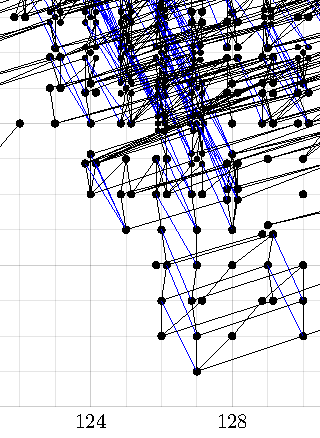
\includegraphics[scale=1.15]{h62-chart-e2.pdf}}
    \columnbreak
    
    \frame{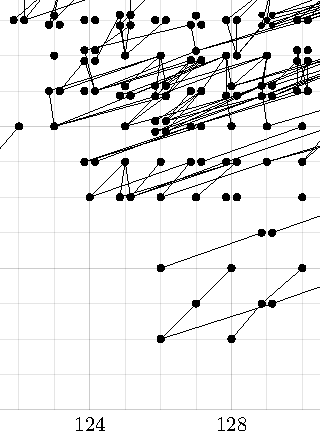
\includegraphics[trim={0cm 0cm 0cm 0.01cm}, scale=1.15]{h62-chart-e3.pdf}}
  \end{multicols}

  \caption{
    In this figure, reproduced from \cite{dexter-chart}, we display the $E_2$-page of the Adams spectral sequence near $h_6^2$ with all $d_2$ differentials and the corresponding $E_3$-page.
  }
  \label{fig:theta6ASS}    
\end{figure}

In \Cref{fig:theta6ASS} we display the Adams spectral sequence for the sphere near the class $h_6^2$.
In this case our knowledge of the $E_2$-page comes from \cite{Bruner2} and the $d_2$ differentials were computed in \cite{dexter} using an implementation of an algorithm of Nassau refining Baues' work on algorithmic computation of Adams $d_2$ differentials. 
% off of the $h_0$-tower on $h_7$ are due to Adams. The $d_2$ differential on $K_0$ can be obtained by applying Bruner's power operation formulas \cite{TODO}
% \[ d_2(D_3(1)) = d_2(\Sq^0(D_3)) = 0, \]
% \[ d_2(K_0) = d_2(\Sq^1(D_3)) = h_0\Sq^2(D_3) = h_0x_{6,94}. \]
% The computation of the relevant Steenrod squares comes from \cite{TODO}.
Applying \cite[Theorem 9.19]{boundaries} we obtain the following lemma.

\begin{lem} \label{lem:theta6-nearby}
  Near $h_{6}^2$ the synthetic homotopy groups satisfy
  \begin{align*}    
    \pi_{124,4}(\clambda^2) &= 0,
    & \pi_{125,4}(\clambda^2) &= \F_2\{ \underline{\lambda} K_0 \},
    & \pi_{126,4}(\clambda^2) &= \F_2\{ \wt{2}^2 \theta_j,\ [D_3(1)] \}, \\
    \pi_{124,3}(\clambda^3) &= 0,
    &  \pi_{125,3}(\clambda^2) &= 0,
    & \pi_{126,3}(\clambda^3) &= \F_2\{ \wt{2} \theta_j,\ \underline{\lambda} [D_3(1)] \}, \\
    &
    & \pi_{125,3}(\clambda^3) &= \F_2\{ \underline{\lambda^2} K_0 \},
    & \pi_{126,2}(\clambda^3) &= \F_2\{ \theta_j,\ \underline{\lambda^2} D_3(1) \},
  \end{align*}
  where $\theta_6$ is a choice of lift of $h_6^2$ to $\clambda^3$, $[D_3(1)]$ is a choice of lift of $D_3(1)$ to $\clambda^2$.
\end{lem}

\begin{rmk}
  The reader may have noticed that, somewhat counter-intuitively, we have chosen to present our examples in the opposite of the usual order. Our reason for doing this is to emphasize that the complexity of $E_2$ page is minimal for the generic element in a $\Sq^0$-family. We expect that this phenomenon is robust.
\end{rmk}


% ---------------------------------------------------------------------------------%
\subsubsection{Power operations}\hfill

The study of power operations in the Adams spectral sequence began with work of Adams, Barratt and Mahowald on the quadratic construction. These ideas were developed further by several others over the next two decades attaining a relatively stable form with Bruner's treatment in \cite{BMMS}.
In order to give our synthetic inductive argument we will need to introduce the synthetic incarnation of this material.\footnote{For a more relaxed introduction see the corresponding chapter in \cite{cookware}}

For the purposes of this paper we only need the simplest example of a power operation: the quadratic construction. This construction, which can be performed in any symmetric monoidal category, takes a map $f$ with target the unit and sends it to the composite
\[ X^{\otimes 2}_{hC_2} \xrightarrow{f^{\otimes 2}_{hC_2}} \o^{\otimes 2}_{hC_2} \xrightarrow{\mu} \o \]
where $\mu$ is the multiplication map provided by the symmetric monoidal structure.

The quadratic construction uses three things: colimits, the symmetric monoidal structure and the commutative algebra structure on the unit. Since a symmetric monoidal left adjoint preserves each of these we learn that the quadratic construction is compatible with such functors. Now consider the following span of symmetric monoidal left adjoints.

\begin{center}
  \begin{tikzcd}
    & \Syn_{\F_p} \ar[r, "\clambda^n \otimes -"] \ar[dl, "\lambda^{-1}"] & \mathrm{Mod}(\Syn_{\F_p}; \clambda^n) \ar[dr, "\clambda \otimes_{\clambda^n} -"] \\
    \Sp & & & \mathrm{Stable}(\A)
  \end{tikzcd}
\end{center}

Although not immediately obvious, the existence of this span essentially encodes (nearly) all known compatibilites between power operations and the Adams spectral sequence. As a demonstration of this we consider the example of a map of synthetic spheres.

\begin{exm} \label{exm:quadratic-basics}
  Suppose we have a map $\alpha : \Ss^{k,s} \to \Ss^{0,0}$.
  Applying the quadratic construction we obtain an associated map
  \[ \Sq(\alpha) : (\Ss^{k,s})^{\otimes 2}_{hC_2} \to \Ss^{0,0}. \]
  The usual filtration on the $C_2$ orbits provides us with a filtration on the source whose associated graded is given by $\Ss^{2k+i,2s-i}$ in its $i^{\text{th}}$ piece. The bottom piece of this filtration is a copy of $\Ss^{2k,2s}$ and composing with the associated inclusion gives $\alpha^2$. Inverting $\lambda$ on $(\Ss^{k,s})^{\otimes 2}_{hC_2}$ gives us $(S^{k})^{\otimes 2}_{hC_2} \simeq \Sigma^k \mathbb{R}\mathrm{P}^\infty_k$ which allows us to work out the attaching maps.\footnote{Since all the attaching maps decrease $s$ they are uniquely determined by what happens on inverting $\lambda$, i.e. by the attaching maps in a stunted projective space.} If we think about $\alpha$ in terms of the class it represents on inverting $\lambda$, then the (changing) values of the $s$-degree of the cells of the quadratic construction are recording lower bounds on the Adams filtrations of power operations.

  Now let's tensor down to $\clambda$.
  The map $\alpha$ now becomes some class $a$ on the Adams $E_2$-page.
  The induced filtration on the quadratic construction now splits because there are no attaching maps of the appropriate degree on the $E_2$-page, so
  \[ \clambda \otimes (\Ss^{k,s})^{\otimes 2}_{hC_2} \simeq \oplus_{i \geq 0} \Sigma^{2k+i,2s-i} \clambda.  \]
  This provides a family of power operations $Q_i$ for $i \geq 0$ where $Q_0(a) = a^2$.
  Examining \cite{May-power-ops} we learn that $Q_i(a) = \Sq^{s-i}(a)$ and $Q_i(a) = 0$ for $i > s$. This tells us that the quadratic construction in the synthetic category unifies the algebraic Steenrod operations on the Adams $E_2$-page with the quadratic construction in the category of spectra.

  Bruner's formulas for Adams differentials on algebraic Steenrod squares can now be read off by examining the $\lambda$-bockstein spectral sequence for $(\Ss^{k,s})^{\otimes 2}_{hC_2}$ and pushing these differentials forward using $\Sq(\alpha)$.
\end{exm}

In general, if we think about $X$ in terms of its bigraded cells, then $\pi_{**}(\nu\F_p/\lambda \otimes X)$ is a bigraded vector space which records the locations of these cells. Then using the fact that $\nu\F_p/\lambda \otimes -$ is symmetric monoidal we can work out the cells needed for $X^{\otimes 2}_{hC_2}$.

\begin{exm}
  Suppose that $X$ has two cells $e_1$ and $e_2$ where $e_j$ is in degree $(k_j,s_j)$.
  Then, $X^{\otimes 2}_{hC_2}$ has cells $Q_i(e_j)$ for $i \geq 0$ in degree $(2k_j+i, 2s_j-i)$ and a single cell $e_1e_2$ in degree $(k_1+k_2,s_1+s_2)$.
\end{exm}

% \begin{lem}
  
% \end{lem}

% \begin{proof}
%   Recall that we have a symmetric monoidal left adjoint
%   \[ i : \Sp^{\Fil} \to \Syn_{\F_p}. \]
%   Since $\Ss^{k,s}$ is the image of $\Ss^k(s)$ from filtered spectra it suffices to note that
%   and in filtered spectra we have $(\Ss^k(s))^{\otimes 2}_{hC_2} \simeq (\Ss^k)^{\otimes 2}_{hC_2}(2s)$.
% \end{proof}

% ---------------------------------------------------------------------------------%

% \subsubsection{old}

% In order to make it easy for us to keep track

% \todo{The stuff here needs to be replaced with something better pretty soon.}
% The arguments in this paper make use of both motvic and synthetic homotopy theory, so we begin with a breif introduction to the relevant formal properties. This introduction is not meant to be complete or thorough with regards to the now vast literature on motivic homotopy theory.
% and is meant to highlight a specific thread For a general introduction to motivic homotopy theory see [reference]. For an introduction centered on its utility in computing homotopy groups of spheres see [reference]. For an introduction to synthetic spectra see [piotr]. For an introduction to the computational properties of synthetic spectra see [cookware].

% Motivic and synthetic homotopy both come from $\mathbb{G}_m$-equivariant deformations of the category of spectra. Such a deformation consists of a category $\Sp_{def}$ satisfying the following properties. \footnote{Given a symmetric monoidal category $\mathcal{C}$ a $\mathbb{G}_m$ equivariant deformation can be defined as a smc $\mathcal{C}_{def}$ equipped with an action of $Qcoh(A1/Gm)$ such that the generic fiber is $\mathcal{C}$. For reasons of $1$-affineness this is the same as a sheaf categories on $A1/Gm$ with generic fiber $\mathcal{C}$.}



% ---------------------------------------------------------------------------------%
% ---------------------------------------------------------------------------------%
\subsection{The inductive approach}
\label{subsec:inductive}\hfill

We now come to the main task of this section: giving a synthetic refinement of the inductive approach to constructing $\Theta_j$. In order to orient the reader we give a brief outline of the main points of the original version of this argument. %\footnote{We also suggest that reader unfamiliar with the original paper \cite{Inductive} read }

\begin{enumerate}
\item Using the hypothesis that $2\Theta_j = 0$ construct a map
  \[ \widehat{\Theta}_j : \Sigma^{2^{j+1}-2} S^0/2 \to S^0 \]
  which is $\Theta_j$ on the bottom cell.
\item Apply the quadratic construction to $\widehat{\Theta}_j$.
  A cell diagram of the source of the resulting map in shown below.
  \begin{center} \begin{tikzcd}[cells={nodes={draw=gray}}, sep=huge]
      {Q_3(a)} \ar[dd, bend left=50, no head, "\eta"] & & Q_1(b) \ar[ddll, no head, "\eta"'] \ar[d, "2", no head] \\
      {Q_2(a)} \ar[dd, bend right=50, no head, "\eta"'] \ar[d, "2", no head] & & {\color{blue} Q_0(b)} \ar[ddll, no head, "\eta"'] \\
      {Q_1(a)}  & & {ab} \ar[dll, "2", no head] \\
      {Q_0(a)}
    \end{tikzcd} \end{center}
  Each cell in this diagram is labelled by its associated Dyer--Lashof operation where $a$ is the bottom cell of the copy of $S^0/2$ and $b$ is the top cell.
\item Composing $D_2(\widehat{\Theta}_j)$ with the inclusion of the bottom cell gives $\Theta_j^2$ and assuming we have a nullhomotopy of this map, the induced map out of the cell indicated in blue will be $\Theta_{j+1}$ and the difference of the pair of cells above it will record a nullhomotopy of $2\Theta_{j+1}$.
\end{enumerate}

Before proceeding further we remark that since inverting $\lambda$ is symmetric monoidal and commutes with colimits any lift of this procedure to the synthetic category (using maps between spheres) will produce something lying over $\Theta_j$. In essence, all that this would do is record an Adams filtration bound on $\Theta_{j+1}$. The next theorem shows that if we linearize with respect to $\clambda^r$, then the same argument works though with a weaker output and an inductive hypothesis which is easier to check (a substantial victory)!

\begin{thm} \label{thm:inductive}
  Fix an $r \geq 2$ and suppose that $\theta_j$ is a lift of $h_j^2$ from $\clambda$ to $\clambda^r$.
  If $2\theta_j = 0$ and $\lambda^2 \theta_j^2 = 0$ in $\pi_{**}(\clambda^r)$,
  then there exists a class $\theta_{j+1}$ lifting $h_{j+1}^2$ to $\clambda^r$ such that $2\theta_{j+1} = 0$ in $\pi_{**}(\clambda^r)$.
  % As a corollary we show that
  % $ d_4(h_j^2) = 0 $
  % for all $j \geq 0$.
  % Suppose that $\theta_j$ is a lift of $h_j^2$ to $\clambda^r$
  % such that $2\theta_j = 0$ and $\lambda^2 \theta_j^2 = 0$,
  % then there exists a $\theta_{j+1}$ in $\clambda^r$ lifting $h_{j+1}^2$
  % such that $2\theta_{j+1} = 0$.
\end{thm}


Throughout the proof of \Cref{thm:inductive} we will work in the symmetric monoidal category of $\clambda^r$-modules.
In order to simplify notation we will use $\o$ to denote $\clambda^r$ (since this is the monoidal unit of the category) and $\o^{k,s}$ to denote $\Sigma^{k,s}\o$.
Before proceeding we pause to point out the key ideas in this proof:
\begin{itemize}
\item Although we work in $\clambda^r$-modules, we can often maintain control over maps at the level of their image under the functor $\clambda \otimes_{\clambda^r} -$.% tensoring down to $\clambda$.
\item In $\clambda$-modules we have good control over the quadratic construction since it induces the action of algebraic Steenrod squares on the cohomology of the Steenrod algebra.% via the algebraic Steenrod squares.
\end{itemize}

\begin{proof}      
  Using a choice of nullhomotopy of $2\theta_j$ we can write down a map
  \[ \widehat{\theta}_j : \o^{2^{j+1}-2,2}/2 \to \o \]
  which is $\theta_j$ on the bottom cell.
  For later use we record the following property (which all choices of $\widehat{\theta}_j$ share):
  \begin{itemize}
  \item[($*$)] Upon tensoring down to $\clambda$ the source of $\widehat{\theta}_j$ splits into two cells.
    The bottom cell maps to $\o$ by $h_j^2$ while the top cell maps to $\o$ by $h_{j+1}$ (as long as $r \geq 2$ and $j \geq 3$).
  \end{itemize}
  To verify ($*$) consider the map of $\lambda$-bockstein spectral spectral sequences induced by $\widehat{\theta}_j$. Label the bottom cell of the source by $a$ and the top cell by $b$. Then, we have $\lambda$-bockstein differential $d_1(b) = h_0 a$. By naturality we learn $d_1(\widehat{\theta}_j(b)) = h_0h_j^2 \neq 0$, which implies $\widehat{\theta}_j(b)$ is the unique non-zero class in $\clambda$ in this degree---$h_{j+1}$\footnote{Note that in this argument we have \emph{proved} the Hopf invariant differentials rather than citing them. The reader should compare this argument with the one which can be made using Bruner's power operations formulas.}.
    
  Applying the quadratic construction (i.e. the functor $(-)^{\otimes 2}_{hC_2}$)
  and postcomposing with the multiplication map on $\o$
  we obtain a map
  \[ \mathrm{Sq}(\widehat{\theta}_j) : (\o^{2^{j+1}-2,2}/2)^{\otimes 2}_{hC_2} \to \o \]
  which is $\theta_j^2$ on the bottom cell.
  Now we make a couple of observations.
  First, we can read off from \Cref{exm:quadratic-basics} that the cell diagram for $(\Ss^{2^{j+1} -2}/2)^{\otimes 2}_{hC_2}$ given above is also a cell structure for $(\o^{2^{j+1}-2,2}/2)^{\otimes 2}_{hC_2}$ where the bigradings of the cells have constant weight (the difference of the two coordinates).
  Second, after tensoring down to $\clambda$ the source splits as a sum of (shifts of) copies of the unit and the Dyer--Lashof operations the cells were labelled by now correspond to the Dyer-Lashof operations (i.e. Steenrod square) they record in $\A$-comodules.
  
  % From the Hopf invariant one differentials we can read off that 
  % any null homotopy of $2\theta_j$ will give a $\widehat{\theta}_j$ that has a $h_j^2$ on the bottom cell and a $h_{j+1}$ on the top cell after tensoring down to $\clambda$.
  As above, we will label the bottom and top cell of $\o^{2^{j+1}-2,2}/2$ as $a$ and $b$ respectively.
  Using our identification of what $b$ does on tensoring down to $\clambda$ from ($*$) we can read off that the cell $Q_0(b)$ in $(\o^{2^{j+1}-2,2}/2)^{\otimes 2}_{hC_2}$ will map to $\o$ via $h_{j+1}^2$.
  This means that if we can remove the cells below this one, then we will have a construction of $\theta_{j+1}$.  
  After including a subcomplex of $(\o^{2^{j+1}-2,2}/2)^{\otimes 2}_{hC_2}$ we obtain a map
  \begin{center} \begin{tikzcd}[cells={nodes={draw=gray}}]
      {Q_1(b) - Q_3(a)} \ar[d, "\lambda\wt{2}", no head] \\
      {Q_0(b)} \ar[dd, no head, "\lambda^2\eta"', bend right] \\
      & \\
      {Q_0(a)} \ar[drr, "\theta_j^2"] \\
      & & {\o}.
    \end{tikzcd} \end{center}
  Note the powers of $\lambda$ which appear in the attaching maps of this cell structure due to the bigradings of the cells. Next we compose this map with the map that pushes that the $\lambda^2$ off the bottom as indicated,
  \begin{center} \begin{tikzcd}[cells={nodes={draw=gray}}]
      {\o^{2^{j+2}-1,1}} \ar[rr, "1"] \ar[d, "\lambda\wt{2}", no head] & & {Q_1(b) - Q_3(a)} \ar[d, "\lambda\wt{2}", no head] \\
      {\o^{2^{j+2}-2,2}} \ar[rr, "1"] \ar[dd, no head, "\eta"', bend right] & & {Q_0(b)} \ar[dd, no head, "\lambda^2\eta"', bend right] \\
      & \\
      {\o^{2^{j+2}-4,2}} \ar[rr, "\lambda^2"] & & {Q_0(a)} \ar[drr, "\theta_j^2"] \\
      & & & & {\o}.
    \end{tikzcd} \end{center}
  Using our assumption that $\lambda^2\theta_j^2$ is nullhomotopic we can factor this composite through $\o^{2^{j+2}-2,2}/2$ via a map which is $h_j^2$ on the bottom cell if we tensor down to $\clambda$. This map is a good choice of $\widehat{\theta}_{j+1}$ and its construction completes the proof.
\end{proof}

\begin{rmk} \label{rmk:theta-ctau-3}
  The condition that $\lambda^2\theta_{j}^2 = 0$ in $\pi_{**}(\clambda^r)$ is implied by asking that $\theta_j^2 =0$ in $\pi_{**}(\clambda^{r-2})$. This means that as a corollary of the fact that $h_j^4 = 0$ for $j \geq 1$ we learn that $h_j^2$ lifts to $\clambda^3$. In particular, $d_2(h_j^2) = 0$ and $d_3(h_j^2) = 0$.
\end{rmk}

\begin{prop} \label{cor:theta-ctau-4}
  There exist lifts $\theta_j$ of the classes $h_j^2$ to $\clambda^4$ with the property that $2\theta_j = 0$ and $\lambda^2 \theta_j^2 = 0$.\footnote{As this is the farthest we lift $h_j^2$ in this paper we will hereafter fix our notation so that $\theta_j$ refers to the classes constructed in this proposition.} In more classical language the first claim is equivalent to saying that $d_4(h_j^2) = 0 $.
\end{prop}

\begin{proof}  
  We proceed by induction on $j$ using \Cref{thm:inductive}.
  The inductive step requires that we check at each step that $\lambda^2 \theta_j^2 = 0$ in $\pi_{**}(\clambda^4)$. In fact we will check the stronger statement that $\theta_j^2 = 0$ in $\pi_{**}(\clambda^2)$.

  For $j \leq 4$ this follows from the fact that $\Theta_j^2 = 0$.
  If $j \neq 7$, then the conclusion follows from the fact that $\Ext_{\A}^{5,2^{j+2} + 1} = 0$ (see Figures~\ref{fig:hj2}, \ref{fig:theta7-8} and \ref{fig:theta6ASS}).

  In the case $j=7$ we must rule out the possibility that $\theta_6^2 = \underline{\lambda} V_0'$ in $\pi_{252,4}(\clambda^2)$.
  In \Cref{lem:theta-4-fold}, in the next subsection, we will give a Toda bracket expression
  $ \theta_6 \in \langle 2, \theta_5, \lambda \theta_5, \wt{2} \rangle$ in $\pi_{126,2}(\clambda^2)$.
  Multiplying by $\theta_6$ and shuffling we have
  \[ \theta_6^2 \in \theta_6 \cdot \langle 2, \theta_5, \lambda \theta_5, \wt{2} \rangle \subseteq \langle \langle \theta_6, 2, \theta_5 \rangle, \lambda \theta_5, \wt{2} \rangle. \]
  
  To proceed we would like to determine the value of the 3-fold $\langle \theta_6, 2, \theta_5 \rangle \in \pi_{189,3}(\clambda^2)$.
  From \Cref{E2 descriptions}(1) we can read off that $\pi_{189,3}(\clambda^2) \cong \Z/4\{[h_6^3]\}$.
  Meanwhile, the synthetic analog of Moss' theorem (see \cite{cookware}) allows us to conclude that the image of $\langle \theta_6, 2, \theta_5 \rangle$ in $\pi_{189,3}(\clambda)$ is zero.
  As a consequence we have  
  \[ \langle \theta_6, 2, \theta_5 \rangle = 2a[h_6^3] \]
  for some $a \in \{0,1\}$.
  Now, with some further shuffling we may conclude that
  \begin{align*}
    \theta_6^2
    &= \langle 2a[h_6^3],\ \lambda \theta_5,\ \wt{2} \rangle 
      \subseteq \langle \wt{2},\ a[h_6^3] \lambda^2 \theta_5,\ \wt{2} \rangle = \langle \wt{2}, 0, \wt{2} \rangle
      = (\pi_{252,3}\clambda^2) \cdot \wt{2} = 0             
  \end{align*}
  where the final step uses \Cref{lem:theta7-theta8-nearby} which tells us $\pi_{252,3}\clambda^2 = 0$.
  \qedhere
  
  %The image of the 3-fold $\langle \theta_6, 2, \theta_5 \rangle$ in $\pi_{189,3}(\clambda)$ is zero by the synthetic analog of Moss' theorem (see \cite{cookware}). As a consequence there is an $x$ in $\pi_{189,4}(\clambda)$ such that $x \underline{\lambda} = \langle \theta_6, 2, \theta_5 \rangle$.
  %Using that we are working $\clambda^2$-linearly, shuffling and simplifying we now get\footnote{Recall that $r_{2,1}$ and $\underline{\lambda}$ are as defined in \Cref{cnstr:bock-maps}.}
  %\begin{align*}
  %  \theta_6^2
  %  &= \langle x \underline{\lambda},\ r_{2,1} \underline{\lambda} %\theta_5,\ \wt{2} \rangle 
  %    \subseteq \langle x,\ \underline{\lambda}r_{2,1} \underline{\lambda} %\theta_5,\ \wt{2} \rangle \\
  %  &= \langle x, 0, \wt{2} \rangle
  %    = x \cdot [\Sigma^{63,0} \clambda,\ \clambda^2]_{\clambda^2} + (\pi_{252,3}\clambda^2) \cdot \wt{2} \\
  %  &= x \cdot 0 + 0 \cdot \wt{2} = 0             
  %\end{align*}
  %where we have used $[-,-]_{\clambda^2}$ to denote homotopy classes of $\clambda^2$-linear maps.
  %The indentifications on the last line come from \Cref{lem:theta7-theta8-nearby} which tells us $\pi_{252,3}\clambda^2 = 0$ and the isomorphism
  %\[ [\Sigma^{63,0} \clambda, \clambda^2]_{\clambda^2} \cong [\Sigma^{63,0} \clambda^2, \mathbb{D}\clambda ]_{\clambda^2} \cong \pi_{64,-2}\clambda = 0. \]
  %Finally, we can use our conclusion that $\theta_j^2$ is zero in $\pi_{**}(\clambda^2)$ to conclude that $\lambda^2\theta_j^2 = 0$ in $\pi_{**}(\clambda^4)$ allowing us to apply \Cref{thm:inductive}.
\end{proof}

Recall from \Cref{cnstr:bock-maps} that $\delta_{4,1}: \clambda \rightarrow \Sigma^{1, -4}\clambda^{3}$ is the cofiber of the restriction map $r_{4,1}: \clambda^4 \rightarrow \clambda$.
% \clambda^n \xrightarrow{r_{n,m}} \clambda^m \xrightarrow{\delta_{n,m}} \Sigma^{1, m-n-1}\clambda^{n-m}


\begin{cor} \label{cor:Hopf-diff}
  For $j \geq 4$ we have $\delta_{4,1}(h_{j+1}) = \wt{2} \theta_{j}$ in $\pi_{**}(\clambda^3)$.
\end{cor}

\begin{proof}
  Examining the map induced by $\widehat{\theta}_j$ on $\lambda$-Bockteins in view of ($*$) in the proof of \Cref{thm:inductive} provides the desired conclusion.
\end{proof}

In the case of $h_6^2$ where we have a spherical class $\Theta_5$ to work with we can provide a more refined statement.

\begin{prop}
  The class $h_6^2$ survives to the $E_{r+3}$-page of the Adams spectral sequence if and only if $\eta\theta_5^2 = 0$ in $\pi_{**}(\clambda^{r})$. 
\end{prop}

\begin{proof}
  Recall from \Cref{cnstr:bock-maps} that we denote the cofiber of the $\lambda$-multiplication map by $\delta_1:\clambda \rightarrow \Sigma^{1, -2} \Ss $, which is the total $\lambda$-bockstein.
   We examine the bottom two cells in the final diagram in the proof of \Cref{thm:inductive}.
  The total $\lambda$-bockstein in the source of this map records the attaching map so
  \[ \delta_1(Q_0(b)) = \lambda \eta Q_0(a). \]
  By naturality we now learn that
  \[ \delta_1(h_6^2) = \lambda \eta \Theta_5^2. \]
  This implies that $h_6^2$ is a permanent cycle if and only if $\lambda \eta \Theta_5^2 = 0$ and more specifically that the $\lambda$-power divisibility of this product records the length of the Adams differential on $h_6^2$.
  % conclude that $\lambda^2\eta\Theta_5^2 = 0$. If the product $\eta\Theta_5^2$ has non-trivial image in $\clambda^{r-2}$, then this would force a $\lambda$-Bockstein differential enforcing this relation. $h_6^2$ is the only possible source of such a differential.

  % For the ``if'' direction we consider the same diagram.
  % Instead of pushing the $\lambda^2$ off the bottom we could have pushed the $\eta$ off the bottom. 
\end{proof}

% \begin{rmk}
%   This proof of this proposition doesn't actually use that we're working in the ``$j=6$'' case.
%   We've 
  
% \end{rmk}
Using this proposition and our knowledge of the synthetic stable stems through topological degree $95$ can give an analysis of the class $\eta \Theta_5^2$ and a corresponding lower bound on the length of an Adams differential on $h_6^2$.

\begin{thm}
  The class $\eta \theta_5^2$ is divisible by $\lambda^6$. In particular, through the previous proposition we learn that $h_6^2$ survives to the Adams $E_9$-page.
\end{thm}

\begin{proof}
Classically, by Corollary~1.10 in \cite{WX}, we have a strictly defined 4-fold Toda bracket for $\Theta_5$:
$$\Theta_5 \in \langle 2, \Theta_4, \Theta_4, 2 \rangle.$$
by Corollary~1.3 in \cite{Xu}, we have $2 \Theta_5 = 0$, therefore
$$\Theta_5^2 \in \Theta_5 \cdot \langle 2, \Theta_4, \Theta_4, 2 \rangle  \subseteq \langle \langle \Theta_5, 2, \Theta_4 \rangle, \Theta_4, 2 \rangle.$$
  
Working synthetically, we also have 
$$2\theta_4 = 0 \in \pi_{30,2}\Ss, \ \theta_4^2=0 \in \pi_{60,4}\Ss, \ 2\theta_5=0 \in \pi_{62,2}\Ss,$$
$$\langle 2, \theta_4, \theta_4\rangle = 0 \in \pi_{61,3}\Ss , \ \theta_5 \in \langle 2, \theta_4, \theta_4, 2 \rangle \subseteq \pi_{62,2}\Ss,$$
by comparing with classical statements and using that these bidegrees are $\lambda$-torsion free. Therefore, 
$$\theta_5^2 \in \theta_5 \cdot \langle 2, \theta_4, \theta_4, 2 \rangle  \subseteq \langle \langle \theta_5, 2, \theta_4 \rangle, \theta_4, 2 \rangle \subseteq \pi_{124,4}\Ss.$$
In order to run the main argument that proves the theorem we now need six additional facts whose proofs we defer for the moment.

\begin{enumerate}
\item $ \pi_{93,3}\Ss \subseteq \lambda^2 \cdot \pi_{93,5}\Ss $.
  In particular, any element in $\langle \theta_5, 2, \theta_4 \rangle \subseteq \pi_{93,3}\Ss$ can be written in the form $\lambda^2 x$, where $x \in \pi_{93,5}\Ss$.\vspace{4pt}
\item For any $x$ as in $(1)$, we have $x \cdot \theta_4 = 0$ in $\pi_{123,7}\Ss$.\vspace{4pt}
\item For any $x$ as in $(1)$, any element in $\langle x, \theta_4, 2 \rangle \subseteq \pi_{124,6}\Ss$ can be written in the form $\lambda^2 z$, where $z \in \pi_{124, 8}\Ss$.\vspace{4pt}
\item $\pi_{124, 8}\Ss \subseteq \lambda \cdot \pi_{124, 9}\Ss$.\vspace{4pt}
\item $\eta \cdot \pi_{124, 9}\Ss \subseteq \lambda \cdot \pi_{125, 11}\Ss$.\vspace{4pt}
\item $\eta \cdot \pi_{31, 1}\Ss \subseteq \lambda^4 \cdot \pi_{32, 6}\Ss$.\vspace{4pt}
\end{enumerate} 

Fact $(1)$ lets us rewrite $\theta_5^2 \in \langle \langle \theta_5, 2, \theta_4 \rangle, \theta_4, 2 \rangle$ as 
$$\theta_5^2 \in \langle \lambda^2 x, \theta_4, 2 \rangle \ \text{for some} \ x \in \pi_{93,5}\Ss.$$
Now, by $(2)$, the bracket $\langle x, \theta_4, 2 \rangle$ is well-defined.
Choose a $y$ in this bracket, then we have
$$\lambda^2 \cdot y \in \lambda^2 \cdot \langle x, \theta_4, 2 \rangle \subseteq \langle \lambda^2 x, \theta_4, 2 \rangle.$$
Since both $\theta_5^2$ and $\lambda^2 \cdot y$ are contained in $\langle \lambda^2 x, \theta_4, 2 \rangle$, their difference belongs to its indeterminacy, which is $\lambda^2 x \cdot \pi_{31,1}\Ss + 2 \cdot \pi_{124,4}\Ss$. Therefore, we have
$$\theta_5^2 \in \lambda^2 \cdot y  + \lambda^2 x \cdot \pi_{31,1}\Ss + 2 \cdot \pi_{124,4}\Ss.$$
Using $(3)$ and $(4)$, we may write $y = \lambda^2 \cdot z = \lambda^2 \cdot \lambda \cdot w$
for some $z \in \pi_{124,8}\Ss$ and $w \in \pi_{124,9}\Ss$. 
Multiplying our expression for $\theta_5^2$ by $\eta$ we obtain
$$\eta \theta_5^2 \in \lambda^2 \cdot \eta \cdot y + \lambda^2 x \cdot \eta \cdot \pi_{31,1} =  \lambda^5 \cdot \eta \cdot w + \lambda^2 x \cdot \eta \cdot \pi_{31,1}\Ss.$$
By $(5)$, $\eta \cdot w$ is $\lambda$-divisible; by $(6)$, $\eta \cdot \pi_{31, 1}$ is $\lambda^4$-divisible. Therefore, $\eta \theta_5^2$ is $\lambda^6$-divisible. 

We now return to proving the six facts from above.\vspace{4pt}
\begin{enumerate}
\item In the 93-stem of the classical Adams sseq both $h_5^3$ and $h_0 h_5^3$ support non-trivial differentials (see \cite{IWX}).
  Synthetically, this means any element in $\pi_{93,3}\Ss$ is divisible by $\lambda^2$.\vspace{4pt}
  %This follows immediately from the classical fact (proved in \cite{IWX}) that in the 93-stem both $h_5^3$ and $h_0 h_5^3$ do not survive to the $E_\infty$-page, so the Toda bracket $\langle \Theta_4, 2, \Theta_5 \rangle$ is detected in Adams filtration at least 5. Synthetically, this means any element in $\langle \theta_4, 2, \theta_5 \rangle \subseteq \pi_{93,3}\Ss$ can be written in the form $\lambda^2 x$, where $x \in \pi_{93,5}\Ss$.
\item Classically, $\langle \Theta_5, 2, \Theta_4 \rangle \cdot \Theta_4 = \Theta_5 \cdot \langle 2, \Theta_4, \Theta_4 \rangle \subseteq \Theta_5 \cdot \pi_{61} = 0$, where the last equality is due to $\pi_{61}S^0 = 0$ (see Theorem~1.9 in \cite{WX}). This means that synthetically $\lambda^2 x \cdot \theta_4$ is $\lambda$-torsion.

From \Cref{fig:theta6ASS}, we know that on the classical Adams $E_2$-page
$$\Ext_{\A}^{s, 123+s} = 0 \ \text{for} \ s \leq 7,$$
$$\Ext_{\A}^{s, 124+s} = 0 \ \text{for} \ s \leq 5.$$
These facts means that synthetically $\pi_{123, 7}\Ss$ contains no non-trivial $\lambda$-torsion elements. Therefore, we must have $x \cdot \theta_4 = 0$ in $\pi_{123,7}\Ss$.\vspace{4pt} 
\item It is clear from the classical Adams $E_2$ and $E_3$-pages in \Cref{fig:theta6ASS} that the synthetic homotopy group 
$$\pi_{124, 6}(\clambda^2) \cong \F_2\{a_{124, 6}, \ \underline{\lambda} a_{124, 7}, \ \underline{\lambda} b_{124, 7}\},$$ 
where $a_{124, 6}$, $a_{124, 7}$, $b_{124, 7}$ are the generators of the classical $E_3$-page in the corresponding degrees. We need to rule out these three elements in $\pi_{124, 6}(\clambda^2)$.

For $a_{124, 6}$, note that $x$ is detected by $h_1g_3$ or it is further $\lambda$-divisible. Then it can be ruled out by the corresponding Massey product 
$$\langle h_1g_3, h_4^2, h_0 \rangle = h_1h_5g_3 = 0 \neq a_{124,6} $$ 
in the Adams $E_3$-page and Moss's theorem (there are no crossing differentials).

For the other two elements, note that both $a_{124, 7}$, $b_{124, 7}$ on the $E_3$-page have nonzero $h_2$-multiples. Therefore, we only need to show that 
$$\nu \cdot \langle x, \theta_4, 2 \rangle \subseteq \pi_{127, 7}(\clambda^2)$$ 
does not contain (a linear combination of) $\nu \cdot \underline{\lambda} a_{124, 7}$ and $\nu \cdot \underline{\lambda} b_{124, 7}$.

In fact, since $h_1g_3 \cdot h_2 = 0$ in $\Ext_{\A}^{6, 96+6}$, and $\Ext_{\A}^{7, 96+7} = 0$, we know that $\nu \cdot x$ is $\lambda^2$-divisible. Therefore, in $\pi_{127, 7}(\clambda^2)$, 
$$\nu \cdot \langle x, \theta_4, 2 \rangle \subseteq  \langle \nu \cdot x, \theta_4, 2 \rangle = \langle 0, \theta_4, 2 \rangle = 2 \cdot \pi_{127, 7}(\clambda^2).$$
Factoring $2$ as $\lambda \wt{2}$ we may use the isomorphism between the Adams $E_3$-page and the image of multiplication by $\lambda$ on $\pi_{**}\clambda^2$ to analyze $2$-divisibility.
In particular, we can read off that $\nu \cdot \underline{\lambda} a_{124, 7}$ and $\nu \cdot \underline{\lambda} b_{124, 7}$ are not 2-divisible in $\pi_{127, 7}(\clambda^2)$
from the fact that $h_2a_{124,7}$ and $h_2b_{124,7}$ are not $h_0$-divisible on the $E_3$-page.\vspace{4pt}
%Inspection of  \Cref{fig:theta6ASS} shows that both $\nu \cdot \underline{\lambda} a_{124, 7}$ and $\nu \cdot \underline{\lambda} b_{124, 7}$ are not 2-divisible in $\pi_{127, 7}(\clambda^2)$. This completes the proof that $\langle x, \theta_4, 2 \rangle$ is $\lambda^2$-divisible.\\

\item This is clear from \Cref{fig:theta6ASS} since the only nonzero element in $\Ext_{\A}^{8, 124+8}$ supports a nonzero $d_2$-differential. Therefore, we have $\pi_{124, 8} \subseteq \lambda \cdot \pi_{124, 9}\Ss$.\vspace{4pt}

\item This is clear from \Cref{fig:theta6ASS} since $h_1 \cdot \Ext_{\A}^{9, 124+9} = 0$. Therefore, we have $\eta \cdot \pi_{124, 9}\Ss \subseteq \lambda \cdot \pi_{125, 11}\Ss$.\vspace{4pt}

\item It is clear from the classical Adams spectral sequence that $\pi_{31, 1}\Ss$ is generated by $\lambda^2 \eta \theta_4$ and $\lambda^4$-multiples. So we only need to show that $\eta \cdot \lambda^2 \eta \theta_4$ is $\lambda^4$-divisible. This is true since it is zero. In fact, classically $\eta^2 \Theta_4 = 0$, so synthetically $\eta^2 \theta_4$ must be a $\lambda$-torsion or zero. For degree reasons, it must be zero. Therefore, we have $\eta \cdot \pi_{31, 1}\Ss \subseteq \lambda^4 \cdot \pi_{32, 6}\Ss$.

\end{enumerate} 
This completes the proof.
\end{proof}


%\begin{proof}
%Classically, by Corollary~1.10 in \cite{WX}, we have a strictly defined 4-fold Toda bracket for $\Theta_5$:
%$$\Theta_5 \in \langle 2, \Theta_4, \Theta_4, 2 \rangle.$$
%by Corollary~1.3 in \cite{Xu}, we have $2 \Theta_5 = 0$, therefore
%\begin{align*}
%    \eta \Theta_5^2 & \in \eta \cdot \langle 2, \Theta_4, \Theta_4, 2 \rangle \cdot \Theta_5 \\
%   & \subseteq  \langle \langle \eta, 2, \Theta_4 \rangle ,  \Theta_4, 2 \rangle \cdot \Theta_5    \\
%    & \subseteq \langle \eta, 2, \Theta_4 \rangle \cdot  \langle \Theta_4, 2, \Theta_5 \rangle 
%  \end{align*}
  
%Working synthetically, this theorem follows from the following five facts.
%\begin{enumerate}
%\item Any element in $\langle \theta_4, 2, \theta_5 \rangle \subseteq \pi_{93,3}$ can be written in the form $\lambda^3 x$, where $x \in \pi_{93,6}$.\\

%\item For any such $x$ in $(1)$, we have $\eta x = \lambda^2 y$ for some $y \in \pi_{94,9}$.\\

%\item For any such $y$ in $(2)$, we have $\langle y, 2, \theta_4 \rangle$ is $\lambda$-divisible.\\

%\item For any such $y$ in $(2)$, we have $y \cdot \pi_{31,1}$ is $\lambda$-divisible.\\

%\item $\lambda^3 \cdot \theta_4 \cdot \pi_{95,6}$ is $\lambda^6$-divisible.\\
%\end{enumerate} 

%In fact, by $(1)$, any element in the expression $\langle \eta, 2, \theta_4 \rangle \cdot  \langle \theta_4, 2, \theta_5 \rangle $ can be written in the form
%$$\lambda^3 x \cdot \langle \eta, 2, \theta_4 \rangle.$$
%In particular, we have
%$$\eta \theta_5^2 \in \lambda^3 x \cdot \langle \eta, 2, \theta_4 \rangle, \ \text{for some} \ x \in \pi_{93,6}.$$
%By $(2)$, we have
%$$\eta \theta_5^2 \in \lambda^3 x \cdot \langle \eta, 2, \theta_4 \rangle \in \lambda^3 \cdot \langle \eta x, 2, \theta_4 \rangle = \lambda^3 \cdot \langle \lambda^2 y, 2, \theta_4 \rangle,$$
%for some $y \in \pi_{94,9}$. On the other hand, we have 
%$$\lambda^5 \cdot \langle y, 2, \theta_4 \rangle \in \lambda^3 \cdot \langle \lambda^2 y, 2, \theta_4 \rangle.$$
%By $(3)$, this expression $\lambda^5 \cdot \langle y, 2, \theta_4 \rangle$ is $\lambda^6$-divisible. By $(4)$ and $(5)$, 
%$$\text{the indeterminacy of} \ \lambda^3 \cdot \langle \lambda^2 y, 2, \theta_4 \rangle = \lambda^3 \cdot \lambda^2 y \cdot \pi_{31,1} + \lambda^3 \cdot \theta_4 \cdot \pi_{95,6}$$ 
%is also $\lambda^6$-divisible. Therefore, every element in this Toda bracket is $\lambda^6$-divisible. In particular, $\eta \theta_5^2$ is $\lambda^6$-divisible. 

%In the rest of the proof, we check the above five facts.\\
%\begin{enumerate}
%\item By Table 11 in \cite{IWX}, classically, the Toda bracket $\langle \Theta_4, 2, \Theta_5 \rangle$ is detected by the element $h_0^3 h_5^3$ in Adams filtration 6. Since this is the surviving element in $\pi_{93}$ with the lowest Adams filtration, we in fact know that all elements in the Toda bracket $\langle \Theta_4, 2, \Theta_5 \rangle$ are detected by $h_0^3 h_5^3$. Therefore, synthetically, any element in $\langle \theta_4, 2, \theta_5 \rangle \subseteq \pi_{93,3}$ can be written in the form $\lambda^3 x$, where $x \in \pi_{93,6}$ and is detected by $h_0^3 h_5^3$.\\

%\item Consider the classical $\eta$-extension on $h_0^3 h_5^3$. In the $E_\infty$-page for $\pi_{94}$, there is an element $h_1x_{93,8}$ in filtration 9. This is the element with the lowest filtration that could receive an $\eta$-extension on $h_0^3 h_5^3$. It follows that $\eta x = \lambda^2 y$ for some $y \in \pi_{94,9}$. Note here we do not claim that $y$ is nonzero, so it could be further $\lambda$-divisible.\\

%\item Combined with the discussion in $(2)$, this follows from the following fact and Moss's theorem
%$$\text{The Massey product} \ \langle h_1x_{93,8}, h_0, h_4^2 \rangle = h_1h_5 x_{93,8} = 0$$
%in the classical Adams $E_3$-page. The last equation follows from relations in Ext in $(t-s,\ s)$-bidegree $(125, 10)$ (see \cite{Bruner2}).\\

%\item This follows from that fact that $\pi_{31,1}$ is $\lambda$-divisible, which follows from the classical fact that all elements in $\pi_{31}$ has Adams filtration higher than 1.\\


%\item By computations in \cite{IWX}, $\pi_{95,6}$ is generated by $h_0h_2g_3$, $\lambda \cdot \Delta h_1h_3h_6$ and elements that are $\lambda^3$-divisible. Therefore, we only need to show 
%\begin{enumerate}
%\item $\lambda^3 \cdot \theta_4$ times a class detected by $h_0h_2g_3$ is $\lambda^6$-divisible.\\
%\item $\theta_4$ times a class detected by $\Delta h_1h_3h_6$ is $\lambda^2$-divisible.\\
%\end{enumerate}
%For $(a)$, classically $h_2g_3$ is a permanent cycle, so $h_0h_2g_3$ detects twice of a class. Synthetically, $h_0h_2g_3$ detects $\wt{2} \cdot h_2g_3$. Then it follows from that fact that $2 \theta_4 = 0$. In fact, we know the wanted expression is zero.\\

%For $(b)$, classically $\Delta h_1h_3h_6$ detects a homotopy class in $\langle \Theta_5, 2, \{\Delta h_1h_3\} \rangle$. Therefore,
%$$\theta_4 \cdot \langle \theta_5, 2, \{\Delta h_1h_3\} \rangle \subseteq \langle \theta_4\theta_5, 2, \{\Delta h_1h_3\} \rangle.$$
%On the other hand, 
%$$\theta_5 \cdot \langle \theta_4, 2, \{\Delta h_1h_3\} \rangle \subseteq \langle \theta_4\theta_5, 2, \{\Delta h_1h_3\} \rangle.$$
%It is clear from classical computations that $\langle \theta_4, 2, \{\Delta h_1h_3\} \rangle$ in $\pi_{63,7}$ is $\lambda^2$-divisible. This is due to classical facts that $h_5 \cdot \Delta h_1h_3 = 0$ in the classical Adams $E_2$-page and that no elements in Adams filtration 8 survive in $\pi_{63}$.
%$$\text{The indeterminacy of} \ \langle \theta_4\theta_5, 2, \{\Delta h_1h_3\} \rangle = \theta_4\theta_5 \cdot \pi_{33,5} + \{\Delta h_1h_3\} \cdot \pi_{93,3}.$$
%By Table 21 in \cite{IWX}, classically $\Theta_4\Theta_5$ is detected by $h_0^2g_3$ in Adams filtration 6. So synthetically, $\theta_4\theta_5$ is $\lambda^2$-divisible. The group $\pi_{93,3}$ is clearly $\lambda^2$-divisible, since classically in $\pi_{93}$, the lowest filtration element that survives is in filtration 6. Therefore, the indeterminacy of this Toda bracket is $\lambda^2$-divisible. We now have showed that every element in this Toda bracket is $\lambda^2$-divisible, so in particular, we have proved $(b)$.
%\end{enumerate} 
%This completes the proof.
%\end{proof}

%\begin{proof}
%  \cite[Theorem ???]{TODO} provides us with an expression of $\Theta_5$ as the 4-fold $\langle 2, \Theta_4, \Theta_4, 2 \rangle$. Using this we can begin shuffling $\eta \Theta_5^2$.
%  \begin{align*}
%    \eta \Theta_5^2
%    &= \Theta_5 \langle 2, \Theta_4, \Theta_4, 2 \rangle \eta 
%    = \langle \langle \Theta_5, 2, \theta_4 \rangle, \Theta_4, 2 \rangle \eta 
%    = \langle \Theta_5, 2, \theta_4 \rangle \langle \Theta_4, 2, \eta \rangle
%  \end{align*}
%  % \todo{The reason I can ignore signs here is that the whole thing is 2 torsion because eta.}
%  The classical 3-fold $\langle \Theta_5, 2, \Theta_4 \rangle$ has been analyzed in \cite{IWX}.
 % Their results can be summarized by saying that there exists a choice of $x$ which maps to $h_0^3h_5^3$ in $\clambda$ such that the value of this 3-fold is $\lambda^3x$. Combining the results of \cite{IWX} and \cite{dexter} we learn that there exists a choice of $y$ so that $\eta x = \lambda^2 y$.
%  The remainder of the proof will consist of verifying that the following manipulations are valid.
%  \begin{align*}
 %   \eta \Theta^2
%    &= \lambda^3 x \langle \eta, 2, \Theta_4 \rangle 
%    = \lambda^3 \langle \lambda^2 y, 2, \Theta_4 \rangle 
%    = \lambda^3 \langle \lambda^2 y, 2, \Theta_4 \rangle \\
%    &\subseteq \lambda^5 \langle y, 2, \Theta_4 \rangle + \lambda^3 \cdot \pi_{95,6}\Ss \cdot \Theta_4 
%    \subseteq \lambda^6 \cdot \pi_{125,11}\Ss 
%  \end{align*}
%  
%  The first thing we need to do is check that $2y = 0$.  
%  Since $\lambda^2y$ is divisible by $\eta$ we know it is $2$-torsion.
%  On the other hand, because $\Delta h_1h_3h_6$ and $h_0h_3g_3$ are permanent cycles the only $\lambda^2$-torsion class in $\pi_{94,9}\Ss$ is also $2$-torsion.
%
%  Next we want to show that $\langle y, 2, \Theta_4\rangle$ is divisible by $\lambda$.
%  To do this we show that it is zero in $\clambda$.
%  We can compute the value of this 3-fold on the $E_2$-page using the synthetic analog of Moss' theorem \cite{cookware} and
%  we get $yh_5 + z h_4^2$ for some class $z$. This is zero since we know from \cite{Bruner2} that no class in $E_2^{10,135}$ is divisible by either $h_5$ or $h_4^2$.
%
%  It remains to show that
%  $ \lambda^3 \cdot (\pi_{95,6}\Ss) \cdot \Theta_4 \subseteq \lambda^6 \cdot \pi_{125,11}\Ss $.
%  We begin by observing that any element of $\pi_{95,6}\Ss$ can be written as a lineary combination of 
%  $\nu \{h_0g_3\}$,  $\lambda\{\Delta h_1h_3h_6\}$ and classes divisible by $\lambda^3$.
%  If we knew that $h_2g_3$ was a permanent cycle, then the first term would be easy to handle because $2\Theta_4 = 0$. In fact, knowing that $d_5(h_2g_3) = 0$ (which was proved in \cite{IWX}) turns out to be enough with a little more work.
%  
%  Let $w$ be a lift of $h_2g_3$ to the homotopy of $\clambda^6$ and let $v$ be a choice of $\{h_0h_2g_3\}$.
%  It will suffice to check that $ (\wt{2} w r_{6,3} - v r_3) \underline{\lambda^3} = 0$. 
%  Consider the class $\wt{2} w r_{6,4} - v r_4$ in $\pi_{95,6}\clambda^4$.
%  This group is generated by $\wt{2}w r_{6,4}$, $\lambda\{\Delta h_1h_3h_6\}$, $\underline{\lambda^3}h_1x_{94,8}$ and $\underline{\lambda^3}h_0h_6l$ and the map $r_{4,3}$ sends the latter two generators to zero.
%  As a consequence we can choose $v$ so that $\wt{2} w r_{6,3} - v r_3 = 0$. %which can be absorbed into the choice of $v$. 

%  % What we need to check is that 
%  % Now we examine the behavior of the reduction mod $\lambda$ maps.
%  % \[ \clambda^5 \to \clambda^4 \]
%  % $\pi_{95,6}\clambda^4$ is generated by $\wt{2}w$, $\lambda\{\Delta h_1h_3h_6\}$, $\underline{\lambda^3}h_1x_{94,8}$ and $\underline{\lambda^3}h_0h_6l$.
%  % $\pi_{95,6}\clambda^3$ is generated by $\wt{2}w$, $\lambda\{\Delta h_1h_3h_6\}$, $\underline{\lambda^3}h_1x_{94,8}$ and $\underline{\lambda^3}h_0h_6l$.
%
%  The final step is showing that
%  $\{\Delta h_1h_3h_6\}\Theta_4$ is divisible by $\lambda^2$.
%  Shuffling the expression for $\{\Delta h_1h_3h_6\}$ as a 3-fold from \cite[???]{IWX} we will obtain the desired divisibility.
%  \begin{align*}
%    \{\Delta h_1h_3h_6\}\Theta_4
%    &= \langle \{\Delta h_1h_3\}, 2, \Theta_5 \rangle \Theta_4 \\
%    &=\langle \{\Delta h_1h_3\}, 2, \Theta_4 \rangle \Theta_5 + \{\Delta h_1h_3\}\langle \Theta_4, 2, \Theta_5 \rangle \\
%    &=\langle \{\Delta h_1h_3\}, 2, \Theta_4 \rangle \Theta_5 + \{\Delta h_1h_3\}\lambda^3 x 
%  \end{align*}
%  The image of the 3-fold $\langle \{\Delta h_1h_3\}, 2, \Theta_4 \rangle$ in $\clambda$ is zero because the middle term $2$ is divisible by $\lambda$ and the indeterminacy vanishes.
%  As a consequence of this we can then read off from \cite{IWX} that $\langle \{\Delta h_1h_3\}, 2, \Theta_4 \rangle$ is divisible by $2$. % $= ?2\{h_1H_1\}$.
%  Since $2 \Theta_5 = 0$ we now have the desired conclusion.

%  % As a consequence after dropping down to $\clambda^5$ we can shuffle
  
%  % \langle 2, \Theta_4, \lambda^3 x \rangle \eta r_6
%  % = 2 \langle \Theta_4, \lambda^3 x , \eta r_6 \rangle
     
%  %  \langle \theta_5, 2, \theta_4 \rangle = \lambda^3 [h_0^3h_5^3]
%  %  \langle \lambda^3 [h_0^3h_5^3], \theta_4, 2 \rangle
%  %  \eta \langle \lambda^3 [h_0^3h_5^3], \theta_4, 2 \rangle
%  %  \langle \eta, \lambda^3 [h_0^3h_5^3], \theta_4 \rangle 2
%  %  \langle 2,  \eta, [h_0^3h_5^3] r_{3} \rangle Dr_{6,3} \theta_4  
%  %  \lambda^2 \bullet \theta_4 Dr_{6,3} = 0
%  %  conclusion $\eta\theta_5^2$ is zero in $\clambda^6$.
%  %  $d_8(h_6^2) = 0$.     
%\end{proof}

% We finish this section by tying up a loose end related to the exception case of $h_7^2$ not covered by the above results.

% \begin{lem} \label{lem:theta-7-ctau-4}
%   The class $\theta_6^2$ is zero in $\clambda^2$.
%   Consequently, there exists a lift $\theta_7$ of $h_j^2$ to $\clambda^4$ with the property that $2\theta_7 = 0$.
% \end{lem}

% \begin{proof}
%   In order to conclude we must rule out the possibility that $\theta_6^2 = \lambda V_0'$.
%   In the next subsection we will give a Toda bracket expression
%   $ \theta_6 \in \langle 2, \theta_5, \lambda \theta_5, \wt{2} \rangle$.
%   Multiplying by $\theta_6$, working $\clambda^2$-linearly, shuffling and simplifying we get
%   \begin{align*}
%     \theta_6^2
%     &\in \theta_6 \langle 2, \theta_5, \lambda \theta_5, \wt{2} \rangle 
%       = \langle \langle \theta_6, 2, \theta_5 \rangle, \lambda \theta_5, \wt{2} \rangle \\
%     &= \langle ?h_0h_6^3 \underline{\lambda}, r_{2,1} \underline{\lambda} \theta_5, \wt{2} \rangle 
%       \subset \langle ?h_0h_6^3, \underline{\lambda}r_{2,1} \underline{\lambda} \theta_5, \wt{2} \rangle \\
%     &= \langle ?h_0h_6^3, 0, \wt{2} \rangle
%       = ?h_0h_6^3 \cdot [\Sigma^{63,0} \clambda, \clambda^2]_{\clambda^2} + (\pi_{252,3}\clambda^2) \cdot \wt{2} \\
%     &= ?h_0h_6^3 \cdot 0 + 0 \cdot \wt{2} = 0             
%   \end{align*}
%   where we have used $[-,-]_{\clambda^2}$ to denote homotopy classes of $\clambda^2$-linear maps.
%   The indentifications on the last line come from \Cref{lem:theta7-theta8-nearby} which tells us $\pi_{252,3}\clambda^2 = 0$ and the isomorphism
%   \[ [\Sigma^{63,0} \clambda, \clambda^2]_{\clambda^2} \cong [\Sigma^{63,0} \clambda^2, \mathbb{D}\clambda ]_{\clambda^2} \cong \pi_{64,-2}\clambda = 0. \]
% \end{proof}





% ---------------------------------------------------------------------------------%
% ---------------------------------------------------------------------------------%
\subsection{A (synthetic) product of $\theta_j$'s}\ 
\label{subsec:product-relation}

Having constructed synthetic lifts $\theta_j$ in $\clambda^4$ we make a short investigation of products among them. More specifically, we show that there is a (non-trivial) product
\[ \theta_j\theta_{j-1} = \underline{\lambda^2} h_0^2g_{j-2} \neq 0 \]
on the Adams $E_4$-page (i.e. in the homotopy of $\clambda^3$)\footnote{We have passed from $\clambda^4$ to $\clambda^3$ here in order to avoid potential extra terms in the product.}. % {and our use of brackets around $4\overline{\kappa}_{j-2}$ indicates that we do not yet know that $\overline{\kappa}_{j-2}$ survives to the $E_4$ page.}.
Though investigating this product may seem unmotivated, as it will turn out, 
knowledge of this product is essentially equivalent to \Cref{thm:main} less the assertion that the differential is non-trivial. % In point of fact, this subsection provides a key input in the proof of \Cref{thm:main} and the section that contains it was created to provide the inputs necessary for this subsection.

\begin{lem}\label{lem:theta-4-fold}
  For $j \geq 5$ and not $7$
  the $\clambda^3$-linear 4-fold
  $ \langle \wt{2}, \lambda \theta_j, \theta_j, 2 \rangle $
  is defined, contains $\theta_{j+1}$ and has no indeterminacy (except in the $j=5$ case where $\underline{\lambda}^2 D_3(1)$ may be in the indeterminacy).
\end{lem}

\begin{proof}
  We start with showing that the 4-fold is defined.
  In \Cref{cor:theta-ctau-4} we showed that $2\theta_j =0$ and $\lambda^2\theta_j^2 = 0$ in $\clambda^4$.
  This means that the 3-folds $\langle \wt{2}, \lambda \theta_j, \theta_j \rangle$ and $\langle \lambda \theta_j, \theta_j, \wt{2} \rangle$ are defined. After tensoring down to $\clambda^3$ we observe that since $\pi_{2^{j+2} - 3, 3}(\clambda^3) = \pi_{2^{j+2} - 3, 2}(\clambda^3) = 0$ as proved in \Cref{lem:near-hj2} and \Cref{lem:theta7-theta8-nearby} both 3-folds are automatically zero.

  In order to unambiguously identify the value of this 4-fold we begin by observing that the reduction map $ \pi_{2^{j+2} -2, 2}(\clambda^3) \to \pi_{2^{j+2} -2, 2}(\clambda)$ is an isomorphism (surjective with kernel $\underline{\lambda}^2D_3(1)$ in the $j=5$ case). As a consequence it will suffice to understand the value of this bracket after reduction to $\clambda$. The desired conclusion can now be obtained using the synthetic version of Moss' theorem for 4-folds \cite{cookware}. 
\end{proof}

As it would be much more involved to argue that $\langle \wt{2}, \lambda \theta_7, \theta_7 \rangle$ is zero in $\pi_{**}(\clambda^3)$ we instead prove a slightly modified form of \Cref{lem:theta-4-fold} in the $j=7$ case.

% In the case where $j = 7$ we 
% Although it seems likely that \Cref{lem:theta-4-fold} remains true in the case $j=7$, since the weaker form suffices for our application of interest we will refrain from tackling the issue of whether $\langle \wt{2}, \lambda \theta_7, \theta_7 \rangle$ is zero.

\begin{lem} \label{lem:theta-8-4-fold}
  In $\clambda^3$ the matric 4-fold
  \[ \left\langle \wt{2}, \begin{pmatrix} \lambda \theta_7 & 0 \end{pmatrix}, \begin{pmatrix} \theta_7 \\ \underline{\lambda^2} \end{pmatrix}, 2 \right\rangle \]
  is defined, contains $\theta_{8}$ and has zero indeterminacy.
\end{lem}

\begin{proof}
  The proof of this lemma is quite similar to previous one, so we will mostly indicate the necessary modification. Each of the 2-fold products are zero as before. 
  The right 3-fold is then defined and lands in a zero group, therefore it suffices to check that the left 3-fold contains zero.
  From \Cref{lem:theta7-theta8-nearby} we know that $\pi_{509,3}(\clambda^3) \cong \Z/2\{ \underline{\lambda^2} V_1'  \}$ which implies that the left 3-fold is equal to its own indeterminacy and therefore it contains zero.
  In order to evaluate the value of this 4-fold we begin with some shuffling,
  \[ \left\langle \wt{2}, \begin{pmatrix} \lambda \theta_7 & 0 \end{pmatrix}, \begin{pmatrix} \theta_7 \\ \underline{\lambda^2} \end{pmatrix}, 2 \right\rangle \subseteq \left\langle \wt{2}, \begin{pmatrix} \lambda \theta_7 & 0 \end{pmatrix}, \begin{pmatrix} \theta_7\lambda \\ 0 \end{pmatrix}, \wt{2} \right\rangle. \]
  
  Next we remove the pair of zero maps through $\Sigma^{1,-3}\clambda$ reducing to an ordinary 4-fold.
  Note that in doing this we must take into account the indeterminacy coming from composites which factor through $\Sigma^{1,-3}\clambda$.
  \[ \left\langle \wt{2}, \begin{pmatrix} \lambda \theta_7 & 0 \end{pmatrix}, \begin{pmatrix} \theta_7\lambda \\ 0 \end{pmatrix}, \wt{2} \right\rangle \subseteq \left\langle \wt{2}, \lambda \theta_7 , \theta_7\lambda , \wt{2} \right\rangle + [\Sigma^{510,2} \clambda^3, \Sigma^{1,-3} \clambda]_{\clambda^3} \cdot [\Sigma^{1,-3} \clambda, \clambda^3]_{\clambda^3} \]
  Using the fact $\clambda^3$ is a free $\clambda^3$-module the adjunction between $\mathbb{S}$-modules and $\clambda^3$-modules allows us to read off that for $f \in [\Sigma^{510,2} \clambda^3, \Sigma^{1,-3} \clambda]_{\clambda^3}$ and $g \in [\Sigma^{1,-3} \clambda, \clambda^3]_{\clambda^3}$ the composite $g \circ f$ depends only on the underlying $\mathbb{S}$-linear composite of $f$ and $g$. 
  From the cofiber sequence 
  $\Ss^{1,-3} \to \Sigma^{1,-3}\clambda \to \Ss^{2,-5}$
  and the fact that $\pi_{1,-3}\clambda^3 = 0$ and $\pi_{2,-5}\clambda^3 = 0$ we can read off that 
  $[\Sigma^{1,-3} \clambda, \clambda^3] = 0$.
  Thus, we may conclude that the composite $g \circ f$ is zero
  and our previous expression simplifies to
  \[ \left\langle \wt{2}, \begin{pmatrix} \lambda \theta_7 & 0 \end{pmatrix}, \begin{pmatrix} \theta_7 \\ \underline{\lambda^2} \end{pmatrix}, 2 \right\rangle \subseteq \left\langle \wt{2}, \lambda \theta_7 , \theta_7\lambda , \wt{2} \right\rangle.\]
  
  % \begin{align*}
  %   &\subseteq \left\langle \wt{2}, \lambda \theta_7 , \theta_7\lambda , \wt{2} \right\rangle \\
  %   &\quad + [\Sigma^{510,2} \clambda^3, \Sigma^{1,-3} \clambda]_{\clambda^3} \cdot [\Sigma^{1,-3} \clambda, \clambda^3]_{\clambda^3} \\
  %   &= \left\langle \wt{2}, \lambda \theta_7 , \theta_7\lambda , \wt{2} \right\rangle + [\Sigma^{510,2} \clambda^3, \Sigma^{1,-3} \clambda]_{\clambda^3} \cdot 0 \\
  %   &= \left\langle \wt{2}, \lambda \theta_7 , \theta_7\lambda , \wt{2} \right\rangle 
  % \end{align*}
  At point this we can conclude as in the previous lemma by observing that the value of this bracket is uniquely identified after reduction to $\clambda$ and then applying the synthetic version of Moss' theorem for 4-folds \cite{cookware}.
\end{proof}

\begin{lem} \label{lem:theta-product-divisible}
  In $\clambda^3$ the product $\theta_{j}\theta_{j+1}$ is divisible by $\wt{2}$ for $j \geq 5$.  
\end{lem}

\begin{proof}
  We begin by handling the case $j \neq 5,7$.
  From \Cref{lem:theta7-theta8-nearby} and \Cref{lem:near-hj2} we know that $\pi_{2^{j+2}-3, 3}\clambda^3 = 0$. This implies that $\langle \theta_j, 2, \theta_j \rangle$ is strictly zero. As a consequence of this relation we are able to shuffle the expression for $\theta_j$ given in \Cref{lem:theta-4-fold} to produce the desired divisibility\footnote{Note that shuffling gives a one-to-one correspondence of values of brackets so indeterminacy issues do not arise in this argument.}
  \[ \langle \wt{2}, \lambda \theta_j, \theta_j, 2 \rangle \theta_j = \wt{2} \langle \lambda \theta_j, \theta_j, 2,  \theta_j \rangle. \]

  In the cases $j=5,7$ we need a different argument to conclude that
  $\langle \theta_j, 2, \theta_j \rangle$ contains zero.
  Since $2\theta_j = 0$ and $\clambda^3$ is an $\E_\infty$-algebra (see \Cref{cnstr:bock-maps})
  %\footnote{As we could not find a construction of the $\E_\infty$-algebra structure on $\clambda^3$ in the literature we include the following brief argument: Using \cite[Remark 4.31]{Pstragowski} we can write $\clambda^3$ as $\tau_{\leq 2}\Ss$ where the truncation with respect to the natural $t$-structure on synthetic spectra (see \cite[\S4.2]{Pstragowski}). The $\E_\infty$-algebra structure on $\clambda^3$ now comes from the fact that the natural $t$-structure is compatible with the tensor product and the fact that the unit is a connective $\E_\infty$-algebra.}
  this bracket contains the product $2 \cdot Q_1(\theta_j)$ where here we are referring to the spherical power operation $Q_1$ on even degree classes first identified by Toda \cite[p.27-28]{TodaBook}. Since all elements of $\pi_{125,3}(\clambda^3)$ and $\pi_{509,3}(\clambda^3)$ are simple 2-torsion we know $2 Q_1(\theta_j) =0$ for $j=5,7$. This finishes the $j=5$ case.
  
  In the case $j=7$ we follow the same basic strategy replacing \Cref{lem:theta-4-fold} with \Cref{lem:theta-8-4-fold}.
  In order to shuffle the 4-fold in this case we need the pair of 3-folds
  \[ \langle \underline{\lambda^2}, 2, \theta_7 \rangle \qquad \text{ and } \qquad  \langle \theta_7, 2, \theta_7 \rangle\]
  to be zero.\footnote{More precisely, we need that we can always pick the nullhomotopy of the product on the right to make the bracket zero.} The first of these brackets is zero since it lands in a zero group and we have already checked the second contains zero.
\end{proof}

The restriction placed on the product of $\theta_j$ and $\theta_{j-1}$ by \Cref{lem:theta-product-divisible} allows us to obtain a corresponding restriction on the Adams differentials on $h_j^3$, which proves \Cref{prop:diff classical}.

\begin{prop} \label{prop:d4-divisible}
  $\delta_{4,1}(h_j^3)$ is divisible by $\wt{2}^2$ for $j \geq 6$.
  Consequently, for $j \geq 6$,
  \begin{enumerate}
  \item $d_2(h_j^3) = 0$,
  \item $d_3(h_j^3)$ is either $0$ or $h_0^2g_{j-2}$ and
  \item $d_4(h_j^3)$ is either $0$ or $h_0^3g_{j-2}$ (if defined).
  \end{enumerate}  
\end{prop}

\begin{proof}
  From \Cref{cnstr:bock-maps} we know that $\delta_{4,1}$ arises as the cofiber of the map of rings $r_{4,1} : \clambda^4 \to \clambda$ and therefore that this map is $\clambda^4$-linear. Using that $\theta_j$ lifts to $\clambda^4$ (by \Cref{thm:inductive}) we may now perform the following manipulations
  \begin{align} 
    \delta_{4,1}( h_j^3 ) = \delta_{4,1}( \theta_j h_j ) = \theta_j \delta_{4,1}(h_j) = \theta_j \cdot \wt{2} \theta_{j-1} \label{eqn:test}
  \end{align}
  where we have used \Cref{cor:Hopf-diff} to identify $\delta_{4,1}(h_j)$.
  Plugging the $\wt{2}$ divisibility of $\theta_j\theta_{j-1}$ from \Cref{lem:theta-product-divisible}
  into this equation completes the proof of the first claim.

  Let $\delta_{4,1}(h_j^3) = \wt{2}^2 \cdot y$ with $y \in \pi_{ 3 \cdot 2^j - 4, 3}\clambda^3$.
  Using our knowledge of the $E_2$-page from \cite{Ext5} (cf. \Cref{E2 descriptions}(1)) together with \Cref{exm:Bruner formula} which lets us lift $g_{j-2}$ to $\clambda^2$ (we denote the lift by $[g_{j-2}]$) we can read off that
  $\pi_{ 3 \cdot 2^j - 4, 3}\clambda^3 \cong \Z/4\{\underline{\lambda}[g_{j-2}]\}$.\footnote{In the case $j=6$ there is an additional summand $\Z/2\{\underline{\lambda^2}(h_7D_3(0))\}$, but this class is $\wt{2}$-torsion and so does not affect the value of $\wt{2}^2 \cdot y$.}
  It follows that $d_2(h_j^3) = 0$ and depending on the value of $y \in \Z/4\{\underline{\lambda}[g_{j-2}]\}$ we fall into one of the following cases
  \begin{itemize}
  \item[(a)] $y$ is a generator and $d_3(h_j^3) = h_0^2g_{j-2}$,
  \item[(b)] $y = 2\underline{\lambda}[g_{j-2}]$, $d_3(h_j^3) = 0$ and $d_4(h_j^3) = h_0^3g_{j-2}$.
  \item[(c)] $y = 0$, $d_2(h_j^3) = 0$, $d_3(h_j^3) = 0$ and $d_4(h_j^3) = 0$.
  \end{itemize}
\end{proof}

Now we can reverse the flow of information.
From \Cref{thm:main} we know that
\[ d_4(h_j^3) = h_0^3g_{j-2} \neq 0, \]
which, when combined with \Cref{eqn:test}, implies:

%\footnote{The reason for ordering things in this somewhat obtuse way is that \Cref{prop:d4-divisible} is used in the proof of \Cref{thm:main}.} %that $\theta_j\theta_{j-1} = \underline{\lambda^2} h_0^2g_{j-2} \neq 0 $ in $\pi_{3\cdot 2^j- 4, 4}\clambda^3$.
% We also know form \Cref{lem:theta-product-divisible} that this product is divisible by $\wt{2}$ and from  our knowledge of the $E_2$-page and \Cref{???} \todo{need that d2 on g is non-zero here.} we can work out that \todo{Make sure this is right.} $\pi_{3\cdot 2^j -4, 3}\clambda^3 \cong \Z/4\{\lambda \overline{\kappa}_{j-2}\}$. Putting all the pieces together we obtain the promised product.

\begin{cor}
  In $\clambda^3$, there is a product relation, $\theta_j\theta_{j-1} = \underline{\lambda^2} h_0^2g_{j-2} \neq 0 $ for $j \geq 6$.
\end{cor}

The family of products in this corollary are one of the first infinite families of hidden products in the Adams spectral sequence. It seems likely that they bear a close relations to the hidden products $\theta_j^2$ which identify the HHR differentials.

%%% Local Variables:
%%% mode: latex
%%% TeX-master: "main"
%%% End:
